\documentclass[oneside]{book}

\usepackage[italian]{babel}
\usepackage{bm}
\usepackage{amsthm}
\usepackage{amsmath}
\usepackage[italiano, linesnumbered]{algorithm2e}
\usepackage{graphicx}
\usepackage{floatrow}
\usepackage{listings}
\usepackage{booktabs}
\usepackage{multirow}
\usepackage[nottoc]{tocbibind}
\usepackage{caption}

\renewcommand{\thesection}{\arabic{chapter}.\arabic{section}}
\renewcommand{\baselinestretch}{1.2}

\addtolength{\skip\footins}{2pc plus 5pt}

\newtheorem{definition}{Definizione}[section]
\newtheorem{exmp}{Esempio}[section]
\newtheorem{assumption}{Assunzione}

\captionsetup{justification=centering}

\setcounter{tocdepth}{3}

\graphicspath{ {./images/} }

\lstdefinelanguage{json}{
    basicstyle=\fontsize{10}{11}\ttfamily,
    stepnumber=1,
    numbersep=8pt,
    showstringspaces=false,
    breaklines=true
}

\title{CTBN}
\date{}
\author{Pietro Epis}

\begin{document}
  \frontmatter

  \begingroup
  \let\clearpage\endgroup
  \null\vspace{\stretch{1}}
  \begin{minipage}{5.3in}
  
    \begin{flushright}
      \begin{em}
        ``If you're afraid of falling,\\then don't look down''
      \end{em}

      \vspace{4cm}

      \begin{em}
        Al Prof. Stella e al Dott. Bregoli, per avermi guidato in questo percorso, per quanto mi hanno trasmesso e 
        per avermi saputo ispirare con la loro passione\\[10pt]
        Ai miei genitori, a Giorgio e ai miei nonni, per il supporto e per la stima che hanno sempre dimostrato nei miei confronti,
        oltre che per la sopportazione\\[10pt]
        A Stefania, Diego, Chiara, Michele, Lorenzo, Syria, Luca L., Luca S., Valeria, Davide e Riccardo, fedeli compagni di montagna, di bici,
        di viaggi, di concerti, di avventure\\e di vita\\[10pt]
        A Giuseppe, Ruben, Simone e Fabio, punti di riferimento in questo percorso universitario
        con cui ho condiviso soddisfazioni e frustrazioni\\[10pt]
        A Webbergate, ovvero Diego e Roberto, per l'opportunità che mi hanno offerto, per la grande disponibilità e per 
        la fiducia dimostrata
      \end{em}
    \end{flushright}
  \end{minipage}
  \vspace{\stretch{2}} \null
\endgroup

  \pagebreak

  \tableofcontents
  \listoffigures

  \mainmatter

  \chapter*{Introduzione}
  \label{chapter_introduzione}
  \addcontentsline{toc}{chapter}{Introduzione}
  \paragraph{}
  Le Reti Bayesiane a Tempo Continuo (CTBN) sono un modello grafico probabilistico nato per rappresentare in modo efficiente sistemi
  dinamici, in evoluzione, sfruttando i concetti fondanti di altri modelli quali le Reti Bayesiane (BN) 
  e i Processi Markoviani a Tempo Continuo (CTMP).\\
  I numerosi domini il cui stato progredisce al trascorrere del tempo (considerato come una quantità continua) costituiscono la naturale applicazione delle CTBN, 
  che permettono di modellarne l'evoluzione nel tempo.
  Un possibile esempio si colloca nel contesto dei mercati finanziari, in cui la quotazione di uno
  stock varia nel tempo e il cui trend è condizionato da diversi fattori, quali l'andamento di altri titoli correlati
  piuttosto che avvenimenti di carattere politico, sociale o commerciale.\\
  Il percorso di stage è stato quindi dedicato all'implementazione di nuove funzionalità all'interno
  della libreria software \textit{PyCTBN}, sviluppata dal \textit{MAD Lab (Models and Algorithms for Data and Text Mining)}
  allo scopo di mettere a disposizione uno strumento completo ed efficiente per utilizzare
  il framework delle reti Bayesiane a tempo continuo. In particolare, i nuovi moduli sviluppati
  vertono sulla generazione randomica di reti e sul processo di campionamento di traiettorie,
  integrando inoltre utility per l'esportazione su file dei dati prodotti.\\
  Questa tesi prevede un capitolo introduttivo (Capitolo \ref{chapter_concetti_preliminari}), strutturato in modo da fornire le definizioni
  fondamentali ed esporre le notazioni di cui si fa uso nei capitoli seguenti, presentando
  poi i modelli da cui derivano le CTBN. Vengono successivamente illustrate le reti a tempo continuo (Capitolo \ref{chapter_ctbn}), 
  partendo dalla definizione formale fino ad arrivare ad una dettagliata trattazione che spiega dal
  punto di vista teorico i concetti e le procedure su cui si basa il lavoro svolto.
  Infine, l'ultimo capitolo (Capitolo \ref{chapter_pyctbn}) ha lo scopo di documentare la libreria PyCTBN, dedicando ovviamente
  particolare attenzione alle nuove classi sviluppate, e di discuterne i risultati
  in termini di efficienza rispetto a velocità di esecuzione e utilizzo della memoria.
  \chapter{Concetti Preliminari}
  \label{chapter_concetti_preliminari}
  \paragraph{}
  Questo capitolo ha lo scopo di introdurre le nozioni fondamentali su cui si
  basano le Continuous Time Bayesian Networks (\textbf{CTBN}).

  \section{Definizioni e Notazione}
  \paragraph{}
  Vengono inizialmente fornite le definizioni essenziali e presentate le notazioni convenzionalmente 
  adottate ed utilizzate nel corso dei capitoli successivi.

  \paragraph{Variabile di Processo} \cite{nodelman-2007}
  Una variabile di processo può essere considerata come una collezione di variabili aleatorie
  indicizzate rispetto al tempo continuo e viene indicata con lettere maiuscole.
  e.g. \textit{E}, \textit{$X_i$}.\\    
  Di conseguenza ci si riferisce alle normali variabili aleatorie con un indice temporale,
  e.g. \textit{$X_{i}(t)$}, \textit{$E_t$}

  \paragraph{Valori delle Variabili}
  Il valore assunto da una variabile è indicato dalla relativa lettera minuscola, e.g. \textit{Z = z}, oppure
  $z_1$, $z_2$, ..., $z_n$ per riferirsi a valori diversi.\\
  L'insieme delle possibili istanze di una variabile \textit{Z} è denotato da \textit{Val(Z)},
  e il numero delle istanze (ovvero la cardinalità dell'insieme) si indica con \textit{Card(Z)}.

  \paragraph{Insiemi di Variabili}
  Insiemi di variabili sono denotati da lettere maiuscole e in grassetto (e.g. \textit{\textbf{E}},
  \bm{$V$}) e i relativi valori con le corrispondenti lettere minuscole (e.g. \textit{\textbf{e}},
  \bm{$v$}).

  \paragraph{Distribuzione di Probabilità}
  La distribuzione di probabilità associata ai valori di una variabile aleatoria \textit{$X(t)$} è denotata
  equivalentemente da \textit{P(X(t))} o da \textit{$P_{x}(t)$}. Nel caso della distribuzione iniziale, ovvero
  quando \textit{t = 0}, si usa scrivere \textit{$P_{x}^{0}$}.\\
  La distribuzione di probabilità condizionata di \textit{X(t)} dato \textit{X(s)} è denotata da
  $P(X(t) \; | \; X(s))$

  \paragraph{Genitori}
  Dato un grafo $\mathcal{G}$, si indica con $\mathbf{Pa}_{\mathcal{G}}(X_i)$ l'insieme dei nodi
  genitori della variabile \textit{$X_i$}.\\
  Similmente, l'insieme dei nodi figli di \textit{$X_i$} è rappresentato da $\mathbf{Cd}_{\mathcal{G}}(X_i)$.

  \paragraph{Densità di un Grafo} \cite{graphs}
  Dato un grafo orientato $\mathcal{G} = (V, \; E)$, dove $V$ sono i nodi ed $E$ gli archi, la densità $d$ è definita come
  il rapporto tra il numero di archi effettivi ($\lvert E \lvert$) e il numero massimo di archi che $\mathcal{G}$ avrebbe 
  se fosse un grafo completo. Formalmente:
  \begin{equation} \label{eq:density}
    d = \frac{\vert E \vert}{\vert V \vert (\vert V \vert - 1)}
  \end{equation}

  \section{Bayesian Networks} 
  Il concetto principale su cui si basano le \textbf{Reti Bayesiane (BN)} è l'indipendenza condizionale, 
  definita come segue.

  \begin{definition}[Indipendenza Condizionale] \cite{conditional-independence}
    Due variabili aleatorie \textit{$B_1$} e \textit{$B_2$} si dicono condizionalmente indipendenti,
    dato un insieme di variabili aleatorie \textit{\textbf{C}}, se e solo se
    \begin{equation}
      P(B_1 \; | \; \bm{C}, B_2) = P(B_1 \; | \; \bm{C})
    \end{equation}
  \end{definition}

  Intuitivamente ciò significa che, per ogni possibile valore delle variabili \textit{\textbf{C}},
  \textit{$B_1$} e \textit{$B_2$} non hanno influenza l'una sull'altra,
  o analogamente che la loro influenza è mediata dalle variabili in \textit{\textbf{C}}.\\
  È ragionevole pensare che la maggior parte delle variabili in una certa rete non abbia un'influenza
  diretta su gran parte delle altre, ma piuttosto che ciascuna variabile sia direttamente condizionata 
  da un sottoinsieme limitato delle altre variabili.\\
  È a questo punto possibile definire formalmente una rete Bayesiana.

  \begin{definition}[Bayesian Network] \cite{bn}
    Una Rete Bayesiana $\mathcal{B}$, definita su un insieme di variabili aleatorie \textit{\textbf{B}},
    è costituita da:
    \begin{itemize}
      \item Un grafo diretto aciclico (DAG) $\mathcal{G}$ in cui ciascun nodo è associato
        ad una variabile \textit{$B_i$} $\in$ \textit{\textbf{B}}
      \item Per ciascuna variabile \textit{$B_i$}, una distribuzione di probabilità condizionata (CPD) 
        $P(B_i \; | \; \mathbf{Pa}_{\mathcal{G}}(B_i))$ che formalizza la dipendenza diretta di \textit{$B_i$}
        dall'insieme dei suoi genitori.
    \end{itemize}
  \end{definition}

  Una rete Bayesiana rappresenta quindi una distribuzione congiunta di probabilità,
  che sfruttando la \textit{Chain Rule} può essere espressa come prodotto di fattori:
  \begin{equation}
    P(B_1, B_2, ..., B_n) = \prod_{i=1}^{n} P(B_i \; | \; \mathbf{Pa}_{\mathcal{G}}(B_i))  
  \end{equation}

  Il grafo $\mathcal{G}$ associato alla rete incorpora anche informazioni riguardanti l'indipendenza
  condizionale tra le variabili, in particolare il fatto che una variabile \textit{$B_i$} $\in$ \textit{\textbf{B}}
  è indipendente dalle variabili che non sono sue discendenti, dato $\mathbf{Pa}_{\mathcal{G}}(B_i)$

  \subsection{Dynamic Bayesian Networks}
  Le \textbf{Reti Bayesiane Dinamiche (DBN)} sono uno strumento che permette di modellare
  processi stocastici a \textbf{tempo discreto} (o \textit{time sliced}).
  Lo stato della rete a ciascun istante di tempo, quindi, è descritto da un insieme
  di variabili aleatorie \textit{\textbf{D}}. 
  Indicizzando gli insiemi di variabili rispetto al tempo, si ottiene che l'intera collezione di variabili è 
  perciò costituita dall'insieme \{$\bm{D_0}$, $\bm{D_1}$, ..., $\bm{D_n}$\},
  dove ciascun elemento $D_i$ denota l'insieme delle variabili della rete all'istante \textit{i}.\\
  Formalmente, una rete Bayesiana dinamica è definita come segue.

  \begin{definition}[Dynamic Bayesian Network]  \cite{nodelman-2007}
    Una rete Bayesiana dinamica è una coppia $\langle\mathcal{B}_0, \mathcal{B}_{2T}\rangle$,
    dove $\mathcal{B}_0$ è la rete Bayesiana basata sulle variabili in $\bm{D_0}$, e $\mathcal{B}_{2T}$
    (chiamato \textbf{2TBN}, 2 Time Slice Bayesian Network) fornisce un modello di transizione dall'istante \textit{i} all'istante \textit{i+1}.\\
    In particolare, $\mathcal{B}_{2T}$ consiste in una rete Bayesiana costituita dalle variabili in $\bm{D_{i+1}}$ 
    condizionate dalle variabili in $\bm{D_i}$.\\
    Gli archi di questa rete vengono classificati in due categorie:
    \begin{itemize}
      \item \textbf{Intra}-time-slice: sono consentiti solo tra variabili appartenenti allo stesso 
        istante temporale, e.g. (X, Y) per X, Y $\in$ \bm{$D_i$}
      \item \textbf{Inter}-time-slice: connettono una variabile nel contesto di un istante temporale ad
        una dell'istante successivo (eventualmente anche la stessa), e.g. (X $\in$ \bm{$D_i$}, X $\in$ \bm{$D_{i+1}$})
    \end{itemize}
  \end{definition}

  \section{Continuous Time Markov Processes}
  Un ulteriore elemento necessario per poter introdurre le reti Bayesiane a tempo continuo consiste nei
  processi Markoviani a tempo continuo (\textbf{Continuous Time Markov Processes}), che derivano dall'aggiunta
  di un'assunzione (assunzione di Markov) ai processi stocastici a tempo continuo.
  
  \begin{definition}[Processo stocastico a tempo continuo] \cite{stochastic-processes}
    Si definisce processo stocastico (o aleatorio) a tempo continuo una collezione di variabili aleatorie
    indicizzate rispetto al tempo $\bm{t \in [0, \infty)}$.\\
    Si consideri la variabile \textit{X} in relazione a tutti i valori di \textit{t} come 
    un'unica variabile (\textbf{Process Variable}).
  \end{definition}

  Definiamo quindi l'assunzione di Markov, da applicare al concetto di processo stocastico a tempo continuo.

  \begin{assumption}[Assunzione di Markov] \cite{ctmp}
    Si assume che, in un processo stocastico, il valore futuro sia indipendente da quello passato, dato il valore presente.\\
    Formalmente, un processo \textit{X} soddisfa l'assunzione di Markov se e solo se
    \begin{equation}
      P(X_{t+\Delta t} \; | \; X_t, X_s) = P(X_{t+\Delta t} \; | \; X_t)
    \end{equation}
    \[
      \forall s, t \; | \; s<t<\infty
    \]
  \end{assumption}

  \paragraph{}
  In altre parole, l'assunzione di Markov implica che la transizione verso un nuovo stato dipenda esclusivamente dallo stato immediatamente precedente,
  e non da come si è giunti ad esso, garantendo quindi la cosiddetta \textit{memoryless property}.
  
  \begin{definition}[Processo Omogeneo] \cite{markov-chains}
    Un processo Markoviano si dice omogeneo se la probabilità di transizione $P(X_{t+1} = b \; | \; X_t = a)$ non dipende
    dall'istante temporale \emph{t} ma esclusivamente dagli stati \emph{a} e \emph{b}.\\
    In un processo di Markov omogeneo, quindi, la probabilità di transizione dallo stato \emph{a} allo 
    stato \emph{b} è costante nel tempo.
  \end{definition}

  \paragraph{}
  È ora possibile fornire la definizione di \textbf{traiettoria}, elemento centrale nel contesto di questa tesi, 
  che verrà ripreso dettagliatamente nel seguito.

  \begin{definition}[Traiettoria]
    Una specifica istanza dei valori di una variabile $X_t$, per ogni \textit{t}, prende il nome di traiettoria.  
  \end{definition}

  \paragraph{Rappresentazione del processo Markoviano}
    Un processo di questo tipo è generalmente definito da una \textit{distribuzione iniziale} e da una
    \textbf{matrice di intensità di transizione}, concetto che sarà fondamentale anche nell'ambito delle
    CTBN.\\
    È previsto che gli elementi della matrice che si trovano sulla diagonale principale abbiano valore negativo, mentre
    gli altri devono essere non negativi.
    Le matrici devono inoltre soddisfare il vincolo tale per cui la somma degli elementi di ciascuna riga sia pari a zero.\\
    Un esempio di matrice è quindi il seguente:

  \[
    Q_X = 
    \begin{bmatrix}
      -q_1 & q_{12} & \dots & q_{1n}\\
      q_{21} & -q_2 & \dots & q_{2n}\\
      \vdots & \vdots & \ddots & \vdots\\
      q_{n1} & q_{n2} & \dots & -q_n
    \end{bmatrix} 
  \]
  \[
    dove \; q_i = \sum_{j \neq i} q_{ij}, \; con \; q_{ij} \geq \; 0 \; \forall \; i, j \in [1, n]
  \]

  \paragraph{}
  L'interpretazione della matrice è che i valori \textit{$q_i$}, ovvero quelli che si trovano sulla
  diagonale, forniscono la probabilità istantanea di lasciare lo stato \textit{$x_i$}, mentre il generico
  elemento in posizione \textit{(i, j)} indica la probabilità istantanea di effettuare una transizione dallo stato \textit{i} allo stato \textit{j}.\\
  Si parla di probabilità istantanea, e non di probabilità in senso assoluto, in quanto 
  i valori che costituiscono una riga non sommano ad uno. È però possibile assimilare un coefficiente al concetto tradizionale di probabilità
  effettuando una normalizzazione rispetto alla riga a cui esso appartiene. Per considerare un
  coefficiente $q_{ij}$ come probabilità $p_{ij}$, quindi, si procede come segue:
  \begin{equation}
    p_{ij} = \frac{q_{ij}}{\sum_{k \in \{1...n\} \setminus i}q_{ik}}
  \end{equation}

  Complessivamente, pertanto, la matrice descrive il comportamento istantaneo del processo \textit{X} rispetto
  allo stato in cui si trova nell'istante corrente.

  \subsection{Conditional Markov Processes}
  \paragraph{}
  Un successivo passo verso la definizione delle CTBN è consentito dal concetto di \textbf{processo Markoviano condizionato} (Conditional Markov Process) \cite{nodelman-2007},
  che è un modello di processo Markoviano \textit{non omogeneo} in cui le intensità di transizione
  variano con il variare del tempo \textit{t}, ma non in funzione di \textit{t}.\\
  Le intensità di transizione di una variabile all'istante \textit{t} dipendono invece dal valore che 
  altre variabili assumono all'istante \textit{t}, con queste ultime che a loro volta evolvono come processi Markoviani.
  
  \subsubsection{Conditional Intensity Matrix}
  \paragraph{}
  Sia \textit{X} una variabile con dominio \textit{Val(X)} = \{$x_1$, $x_2$, ..., $x_n$\} e sia
  $\mathbf{P} = \mathbf{Pa}(X)$.\\
  \textit{X} evolve nel tempo come processo Markoviano le cui variazioni sono condizionate dallo
  stato delle variabili in $\mathbf{P}$, che a loro volta evolvono al variare del tempo.\\
  La necessità di esprimere questa dipendenza introduce il concetto di Conditional Intensity Matrix (\textbf{CIM}),
  sulla base delle matrici di intensità già mostrate. Una CIM, infatti, è sostanzialmente composta da un insieme
  di matrici di intensità, una per ciascuna istanza \textbf{p} delle variabili \textbf{P}.\\
  Nel caso limite in cui \textit{X} non ha genitori, la sua CIM corrisponde esattamente ad una semplice
  matrice di intensità.\\
  Una notazione che evidenzia la variazione dei parametri della matrice in funzione dei valori di 
  \textbf{p} è la seguente (in cui chiaramente valgono gli stessi vincoli sui valori della diagonale): 

  \vspace{6mm}
  \[
    Q_{X|P} = 
    \begin{bmatrix}
      -q_1(P) & q_{12}(P) & \dots & q_{1n}(P)\\
      q_{21}(P) & -q_2(P) & \dots & q_{2n}(P)\\
      \vdots & \vdots & \ddots & \vdots\\
      q_{n1}(P) & q_{n2}(P) & \dots & -q_n(P)
    \end{bmatrix} 
  \]
  \vspace{6mm}

  Una \textit{CIM}  è sempre di forma quadrata, e in particolare di dimensione pari al numero di stati
  che la variabile \textit{X} a cui essa è associata può assumere, ovvero la sua cardinalità \textit{Card(X)}.

  \chapter{Continuos Time Bayesian Networks}
  \label{chapter_ctbn}
  \section{Introduzione}
  \paragraph{}
  In questo capitolo viene presentato il modello delle \textbf{Continuous Time Bayesian Networks (CTBN)} e la sua semantica.\\
  Questo modello è costruito sulla base dei concetti esposti in relazione ai \textit{Processi Markoviani a Tempo Continuo},
  riprendendo inoltre la definizione delle \textit{Bayesian Networks} per sfruttarne la rappresentazione compatta.
  
  \paragraph{}
  Nonostante anche le \textit{Dynamic Bayesian Networks} consentano di modellare una rete che progredisce
  nel tempo, tracciandone lo stato ad istanti successivi, esse non rappresentano esplicitamente il concetto del tempo. 
  Nelle \textit{DBN}, infatti, le variabili sono indicizzate stabilendo un ordinamento, ma non è presente alcun riferimento 
  all'istante temporale effettivo a cui esse appartengono. 
  Conseguentemente, tale prerogativa fa sì che nelle reti dinamiche il tempo venga regolarmente suddiviso in intervalli di ampiezza costante, 
  comportando limitazioni significative all'efficacia e all'applicabilità di tale modello, precludendo ad esempio la possibilità che i diversi processi 
  evolvano con granularità temporali differenti, oppure che le osservazioni avvengano ad intervalli irregolari.\\
  L'elusione di queste limitazioni richiederebbe di rappresentare l'intero sistema con la più piccola granularità
  possibile, implicando quindi di includere anche istanti temporali intermedi in cui non è occorsa nessuna
  osservazione.\\
  Le CTBN consentono perciò di superare tali limiti, basandosi sui processi Markoviani ma mantenendo
  le idee fondanti delle \textit{DBN}.

  \begin{definition}[Continuous Time Bayesian Networks] \cite{nodelman-2002}
    Sia \textit{\textbf{X}} un insieme di variabili $X_1, X_2, ..., X_n$, dove ciascuna variabile rappresenta
    un processo Markoviano a tempo continuo.\\
    Una Continuous Time Bayesian Network $\mathcal{N}$ su \textit{\textbf{X}} è definita da:
    \begin{itemize}
      \item Una distribuzione iniziale $\mathcal{B}_0$, rappresentata come rete Bayesiana
      \item Un modello di transizione, costituito da:
      \begin{itemize}
        \item Un grafo $\mathcal{G}$ sulle variabili in \textit{\textbf{X}}
        \item Una \textit{Conditional Intensity Matrix} $Q_{X|Pa(X)}$ per ciascuna variabile in \textit{\textbf{X}}
      \end{itemize}
    \end{itemize}
  \end{definition}

  \paragraph{}
  Come già anticipato in precedenza nel contesto dei \textit{Conditional Markov Processes},
  la presenza di un arco da X ad Y rappresenta la dipendenza delle intensità di transizione
  di Y dai valori assunti da X.\\
  È importante sottolineare come nelle CTBN, a differenza delle reti Bayesiane classiche,
  non sia necessario imporre che il grafo sia aciclico.
  Infatti, anche se esiste un arco \textit{(X, Y)} che denota l'influenza di Y nell'evoluzione di X,
  è concettualmente ammissibile che la transizione di Y possa dipendere a sua volta da X,
  implicando l'esistenza di un arco \textit{(Y, X)}.  

  \section{Campionamento}
  \paragraph{}
  Il modello delle CTBN prevede un'assunzione fondamentale, la quale impone che una ed una sola variabile 
  possa effettuare una transizione verso un nuovo stato in uno specifico istante temporale. 
  Questo vincolo ha un'importante implicazione dal punto di vista semantico, dal momento che può essere visto come 
  la formalizzazione del fatto che ciascuna variabile riflette un aspetto della realtà atomico e distinto rispetto alle altre variabili.
  Non sarebbe quindi né significativo, né realistico, usare le CTBN per modellare un dominio in cui più variabili possono cambiare stato nello stesso istante.
  
  \paragraph{}
  Dopo aver introdotto tutte le definizioni e i concetti teorici necessari, viene ora mostrata,
  in forma di pseudo-codice, la procedura che costituisce il cuore del lavoro svolto durante lo stage,
  e conseguentemente di questa tesi, che ha lo scopo di simulare l'evoluzione dello stato delle variabili della rete,
  campionando casualmente una \textit{traiettoria}.

  \begin{algorithm}
    \DontPrintSemicolon
    \SetKwFunction{FMain}{CTBN\_Sample}
    \SetKwProg{Fn}{Procedure}{:}{}
    \Fn{\FMain{$t_{end}$}}{
      t $\leftarrow$ 0, 
      $\sigma$ $\leftarrow$ $\emptyset$\;
      \;
      \ForEach{$\textit{X} \in \mathbf{X}$}
        {Scegli $x(0)$ dato $\bm{\theta}^{\mathcal{B}}_{X \; | \; \mathbf{Pa}_{\mathcal{B}}(X)}$}
      \;
      \While {true}{
        \ForEach{$\textit{X} \in \mathbf{X}$}{
          \uIf{Time(X) \textbf{is} \textit{undefined}}{
            $\Delta t$ $\leftarrow$ $random\_exponential(q_{x(t) \; | \; u_x(t)})$\;
            $Time(X)$ $\leftarrow$ t + $\Delta t$
          }
        }
        \;
        $X_{tr}$ $\leftarrow$ $arg \; min_{Y \in \bm{X}}$[Time(Y)]\;
        t $\leftarrow$ Time($X_{tr}$)\;
        \;
        \eIf{$t \geq t_{end}$}{
          \KwRet $\sigma$\;
        }{
          $x_{tr}(t) \leftarrow random\_multinomial(\bm{\theta}_{x(t) \; | \; u_x(t)})$\;
          Aggiungi $\langle t, x_1(t), x_2(t), ..., x_{tr}(t), ..., x_n(t) \rangle$ a $\sigma$
        }
        \;
        
        \ForEach{$Y \in \mathbf{Cd}(X_{tr}) \cup X_{tr}$}{
          $Time(Y) \leftarrow undefined$\;
        }
      }
    }
    
    \captionof{algocf}{Procedura CTBN\_Sample}
    \label{alg:ctbn_sample}
  \end{algorithm}

  Il metodo \textit{CTBN\_Sample}, quindi, restituisce come risultato una traiettoria che parte dall'istante $t_0 = 0$
  e tale per cui l'istante temporale associato all'ultima occorrenza che è stata campionanta è minore o uguale al parametro $t_{end}$
  specificato.\

  \subsection{Interpretazione dello pseudo-codice}
  Questa sezione si occupa di analizzare e spiegare le istruzioni dell'Algoritmo \ref{alg:ctbn_sample}.\\
  La procedura si occupa, in fase di inizializzazione nelle righe da \textit{2} a \textit{6}, 
  di assegnare il valore $0$ alla variabile $t$, che rappresenta l'istante temporale corrente, e di definire la traiettoria $\sigma$
  come insieme vuoto $\emptyset$.\\
  Si è deciso di rappresentare la traiettoria come un insieme, quindi senza un ordinamento, in quanto
  ciascun elemento appartenente ad esso include l'informazione temporale corrispondente. 
  Una rappresentazione equivalentemente consisterebbe in una sequenza ordinata di n-uple.\\
  A riga \textit{5} si valorizzano le variabili all'istante $t=0$, infatti $\theta^{\mathcal{B}}_{X \; | \; \mathbf{Pa}_{\mathcal{B}}(X)}$
  indica la distribuzione di probabilità iniziale della variabile $X$ dati i suoi genitori.\\ 
  La parte più significativa della procedura, ovvero il campionamento vero e proprio della 
  traiettoria, è data dalla ripetizione del blocco di istruzioni definite nel corpo
  del ciclo \textit{while} che inizia a riga \textit{8}.\\
  Premesso che con $Time(X)$ ci si riferisce all'istante temporale in cui $X$ effettuerà la prossima transizione di stato,
  la prima operazione che viene svolta all'inizio di ciascuna iterazione ha lo scopo di determinare $Time(X)$
  per ogni variabile $X$ tale per cui esso non sia già definito. Come verrà spiegato successivamente,
  l'insieme delle variabili il cui tempo di transizione è indefinito è costituito
  dalla variabile che ha cambiato stato all'iterazione immediatamente precedente a quella corrente, unitamente alle 
  variabili che dipendono da essa (in altre parole le sue figlie).\\
  Per calcolare $Time(X)$ si somma al tempo corrente $t$ un valore $\Delta t$ estratto in 
  modo casuale da una distribuzione esponenziale di parametro $q_{x(t) \; | \; u_x(t)}$.
  La distribuzione esponenziale si addice a questo scopo (e in generale ai domini in cui si rappresenta il tempo rimanente
  prima che si verifichi un evento) in quanto gode della proprietà di \textit{assenza di memoria},
  che stabilisce che il tempo trascorso non influisce sulla probabilità che l'evento si verifichi.
  Tale proprietà viene formalizzata come segue:
  \begin{equation}
    P(X > m + n \; | \; X > m) = P(X > n)  
  \end{equation}
  Questo paramentro consiste chiaramente nel coefficiente della CIM che si trova alla
  riga associata allo stato attuale della variabile, in corrispondenza della diagonale.
  Come spiegato nella trattazione sulle \textit{CIM}, l'interpretazione di questo coefficiente è
  riconducibile alla probabilità di lasciare lo stato corrente.\\
  Acclarato che $Time(X)$ risulta ora definito per ogni nodo appartenente alla rete,
  si procede ad identificare la variabile che verrà coinvolta per prima in un cambio di stato, ovvero quella 
  caratterizzata dal minor tempo di transizione associato. Ciò è formalizzato attraverso 
  l'espressione a riga \textit{15}, denotando con $X_{tr}$ la variabile identificata per la transizione.\\
  Si simula quindi un avanzamento nel tempo, un'evoluzione, aggiornando l'istante temporale corrente
  all'istante in cui avviene la transizione della variabile prescelta. A questo punto,
  se questa progressione implicasse il raggiungimento o eventualmente il superamento del tempo massimo
  $t_{end}$, la procedura terminerebbe ritornando la traiettoria generata fino a quel momento.
  Il raggiungimento del tempo massimo stabilito costituisce quindi la condizione di uscita del loop di generazione 
  della traiettoria.\\
  Se invece questa condizione non è verificata, si procede all'effettivo cambio di stato della
  variabile identificata in precedenza. 
  Nel caso generale di variabili con cardinalità \textit{n}, il nuovo valore viene
  determinato casualmente estraendolo da una multinomiale con parametri $\theta_{x(t) \; | \; u_x(t)}$.
  La distribuzione multinomiale consiste in una generalizzazione della distribuzione binomiale, in cui le variabili
  possono assumere solo i valori 0 e 1, al caso in cui ciascuna variabile può assumere $k$ diversi valori.
  I coefficienti $\theta_{x(t) \; | \; u_x(t)}$ utilizzati per la multinomiale sono interpretabili come l'insieme di probabilità
  che la variabile $X$ effettui una transizione verso ciascuno dei possibili stati, dato l'insieme delle istanze dei genitori $u_x(t)$. 
  Da un punto di vista pratico, questi coefficienti costituiscono la riga della \textit{CIM} corrispondente all'attuale valore della variabile,
  previa normalizzazione (in modo che la somma dei coefficienti che la compongono sia 1).\\
  Poiché la variabile che compie la transizione non può mantenere lo stato corrente, è necessario avere cura di 
  azzerare la probabilità che lo stato estratto corrisponda a quello attuale (ovvero il valore proveniente dal coefficiente che si trova sulla diagonale).\\
  Questo accorgimento, unitamente all'identificazione di una sola variabile per ciascuna iterazione, è necessario per soddisfare 
  il vincolo precedentemente introdotto in relazione al fatto che esattamente una variabile cambi stato in un dato istante.\\
  È possibile asserire che nel caso particolare di variabili binarie, ossia con cardinalità 2, la transizione è 
  implementabile semplicemente negando lo stato corrente tramite la formula

  \begin{equation}
    x_{tr}(t) = 1 - x_{tr}(t-1)  
  \end{equation}

  Una volta realizzata la transizione effettiva di $X_{tr}$, si ottiene una nuova istanza che viene aggiunta alla traiettoria,
  interpretabile come una descrizione dello stato di $\bm{X}$, ovvero di tutte le variabili appartenenti
  alla rete, all'istante temporale corrente \textit{t}. Questa rappresentazione
  viene implementata come una sequenza ordinata in cui si pone in prima posizione
  l'istante temporale a cui si riferisce la situazione descritta, seguito dallo
  stato attuale di tutte le \textit{n} variabili della rete (riga \textit{22}).\\
  Il \textit{foreach} finale a riga \textit{25} si occupa di reimpostare ad \textit{undefined} 
  il tempo di transizione della variabile $X_{tr}$ che ha appena cambiato stato nell'iterazione corrente,
  e di tutte le variabili che hanno un arco entrante che parte da essa, quindi dipendenti.
  Ciò permette di fare in modo che alla successiva iterazione venga determinato un nuovo
  istante temporale per la transizione di queste variabili, come illustrato in precedenza.\\
  L'implementazione effettiva integrata nella libreria \textit{PyCTBN}
  è stata arricchita di alcune estensioni e funzionalità, che verranno descritte
  nella sezione dedicata, la quale si occupa inoltre di mostrare in termini attuativi
  quanto introdotto con lo pseudo-codice.    
  \chapter{PyCTBN}
  \label{chapter_pyctbn}
  \paragraph{}
  La libreria \textbf{PyCTBN} è stata sviluppata allo scopo di fornire uno strumento completo,
  estensibile e soprattutto efficiente per operare agevolmente con il modello delle
  \textit{Continuous Time Bayesian Networks}. La libreria implementa le funzionalità
  relative all'importazione dei dati, all'apprendimento delle strutture e dei
  parametri.\\
  Nel contesto dell'attività di stage sono stati sviluppati classi e metodi volti ad
  integrare nel framework già esistente funzionalità quali il campionamento di traiettorie e la 
  generazione casuale della struttura di una rete e delle relative \textit{CIM}.\\
  Questo capitolo ha lo scopo di fornire preliminarmente un'introduzione generale a PyCTBN, alla sua
  struttura e alle scelte implementative adottate, fornendo poi una descrizione approfondita
  delle nuove funzionalità introdotte.

  \section{Tecnologie e Linguaggi utilizzati}
  \subsection{Python}
  PyCTBN è stata realizzata in \textbf{Python 3}, linguaggio utilizzabile con licenza
  \textit{Open Source}, che è stato inizialmente introdotto all'inizio degli anni 90 e 
  largamente diffuso oggi nell'ambito di applicazioni scientifiche, dell'intelligenza artificiale e della data science.\\
  Tra i vantaggi che ne hanno permesso la diffusione, i più significativi sono la
  presenza di una fiorente community di sviluppatori, che implica la disponibilità di una
  vastissima collezione di librerie e package, e la compattezza della sintassi.\\
  Inoltre, Python viene considerato multi-paradigma, in quanto permette l'adozione
  sia della programmazione procedurale che della \textit{Object Oriented Programming}.\\
  Si tratta però di un linguaggio interpretato, caratteristica da cui deriva il principale 
  svantaggio di Python, vale a dire una riduzione delle prestazioni in termini di velocità
  se raffrontate con quelle conseguibili con linguaggi compilati quali \textit{C} e \textit{C++}.

  \paragraph{}
  Le librerie su cui è stato basato lo sviluppo delle nuove funzionalità sono:
  \begin{itemize}
    \item Pandas: libreria che offre strumenti per l'analisi e la manipolazione di dati,
      come ad esempio la possibilità di utilizzare DataFrame. \cite{pandas}
    \item NumPy: libreria che implementa funzioni per il calcolo scientifico e la
      gestione di array di grandi dimensioni. È sviluppata in C e Pyhton, motivo per
      il quale consente di raggiungere prestazioni nettamente superiori a quelle 
      ipotizzabili con le tradizionali liste. \cite{numpy}
  \end{itemize}

  \subsection{Versioning}
  Per il controllo della versione del progetto si è scelto di utilizzare \textbf{Git},
  facendo riferimento alla seguente repository remota su \textbf{GitHub}:
  \begin{center}
    https://github.com/pietroepis/PyCTBN
  \end{center}
  
  È stata inizialmente creata una \textit{fork} del progetto originale \footnote{https://github.com/madlabunimib/PyCTBN}, aggiungendo poi
  un branch \textit{trajectory-generation}.

  \section{Formato dei dati}
  \paragraph{}
  Per la rappresentazione e il salvataggio delle informazioni relative alle \textit{CTBN},
  è stato sfruttato il formato \textbf{JSON} (JavaScript Object Notation), definendo convenzionalmente una struttura
  che renda agevoli le operazioni di importazione ed esportazione.\\
  Per quanto riguarda la struttura del dataset, nell'implementazione attuale di PyCTBN 
  si è deciso di mantenere lo stesso standard previsto dalla libreria \textbf{CTBN-RLE} \cite{package},
  fruibile tramite il linguaggio \textit{R}. La natura estensibile di PyCTBN, tuttavia,
  permette di adattare agevolmente a formati alternativi le procedure di input/output,
  senza influire sulla \textit{business logic}.

  \paragraph{}
  Le informazioni di interesse necessarie per costituire una descrizione completa della rete sono:
  \begin{itemize}
    \item Variabili: sono caratterizzate da una \textit{label} (il nome della variabile) e dalla cardinalità
      (chiave \textit{variables} dell'oggetto JSON)
    \item Struttura della rete: consiste nell'elenco degli archi che collegano la variabili della rete
      (chiave \textit{dyn.str})
    \item Conditional Intensity Matrices: ciascuna variabile possiede tante \textit{CIM} quante sono le 
      combinazioni ottenibili dagli stati che possono assumere i suoi nodi genitore (chiave \textit{dyn.cims})
    \item Traiettorie: elenco di \textit{zero o più} traiettorie generate sulla rete descritta (chiave \textit{samples})
  \end{itemize}

  Viene ora fornito un esempio di rappresentazione di una \textit{CTBN} nel formato JSON
  adottato.
  
  \begin{figure}[H]
    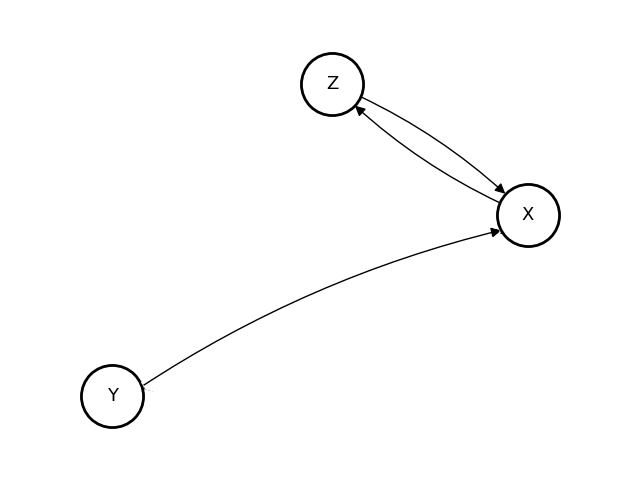
\includegraphics[width = 6cm]{network_graph}
    \centering
    \caption{Network Graph}
    \label{fig:network_graph}
  \end{figure}

  \begin{exmp}[Rappresentazione di una \textit{CTBN}]
    Si supponga di voler memorizzare in formato JSON le informazioni relative alla rete
    basata sul grafo mostrato in \textit{Figura \ref{fig:network_graph}}, costituita quindi dalle variabili $X$, $Y$ e $Z$,
    tutte con cardinalità 3 (possono assumere i valori 0, 1 e 2).\\
    La struttura corrispondente è la seguente:

    \begin{lstlisting}[language=json]
      {
        "variables": [
          {"Name": "X", "Value": 3}, 
          {"Name": "Y", "Value": 3}, 
          {"Name": "Z", "Value": 3}
        ],
        "dyn.str": [
          {"From": "X", "To": "Z"}, 
          {"From": "Y", "To": "X"}, 
          {"From": "Z", "To": "X"}
        ],
        "dyn.cims": {
          "X": {
            "Y=0,Z=0": [
              {"0": -2.5226, "1": 2.495, "2": 0.0276}, 
              {"0": 1.822, "1": -2.8677, "2": 1.0458}, 
              {"0": 0.1172, "1": 2.4934, "2": -2.6106}
            ], 
            "Y=1,Z=0": [
              {"0": -2.6396, "1": 1.0499, "2": 1.5898}, 
              {"0": 0.8389, "1": -1.3058, "2": 0.4669}, 
              {"0": 1.1103, "1": 0.4139, "2": -1.5243}
            ], 
            ...
            "Y=2,Z=2": [
              {"0": -1.3253, "1": 1.315, "2": 0.0103}, 
              {"0": 0.8795, "1": -1.7377, "2": 0.8582}, 
              {"0": 0.4281, "1": 1.7831, "2": -2.2112}
            ]
          },
          "Y": {...},
          "Z": {...}
        },
        "samples": [
          [
            {"Time": 0, "X": 0, "Y": 0, "Z": 0}, 
            {"Time": 0.5237, "X": 0, "Y": 1, "Z": 0}, 
            {"Time": 0.5962, "X": 0, "Y": 0, "Z": 0},
            ...
            {"Time": 1508.1999, "X": -1, "Y": -1, "Z": -1}
        ]
      }
    \end{lstlisting}
  \end{exmp}

  \paragraph{}
  La struttura mostrata nell'esempio è piuttosto autoesplicativa, ma occorre aggiungere alcune precisazioni
  per completezza. L'oggetto indicizzato da \textit{dyn.cims} include a sua volta una chiave 
  per ciascuna variabile, per contenere le CIM relative ad essa. 
  Ricordando che la variabile $X$ ha due archi entranti, provenienti dalle variabili
  $Y$ e $Z$, si può notare come le CIM relative ad $X$ siano state espresse in funzione
  degli stati dei nodi genitore, enumerando tutte le possibili combinazioni.\\
  Nell'esempio sono state incluse per brevità le informazioni concernenti le CIM della sola
  variabile $X$ (la più significativa, avendo due archi entranti), tuttavia è importante sottolineare che l'oggetto 
  relativo alla variabile $Y$ conterrebbe una sola matrice, poiché dal momento che tale variabile non possiede nessun arco entrante
  i suoi valori non dipendono da nessun nodo genitore.\\
  L'interpretazione dell'array con cui viene rappresentata una CIM, prevede che
  l'\textit{i-esimo} elemento dell'array si riferisca allo stato $x = i$ della variabile (considerando 
  un indicizzazione \textit{0-based}). 
  Le chiavi di questo oggetto indicano poi lo stato verso cui avviene la transizione, 
  consentendo di ottenere il coefficiente associato.\\
  Esemplificando, il coefficiente relativo alla probabilità che la variabile $X$, nel caso in cui $Y=0$ e $Z=0$,
  effettui una transizione dallo stato \textit{1} allo stato \textit{2} è quindi 1.0458.\\
  Per quanto riguarda le traiettorie contenute in \textit{samples}, che come detto 
  possono essere molteplici, l'unica puntualizzazione necessaria è volta ad enunciare la convenzione tale per cui
  ciascuna traiettoria deve terminare con un'osservazione fittizia in cui tutte le variabili hanno valore -1.\\
  Lo standard adottato prevede che un file possa contenere la descrizione di più reti distinte,
  quindi il dataset in formato \textit{json} si presenta come un array di oggetti del formato mostrato 
  nell'\textit{Esempio 3.2.1}.

  \section{Package}
  \begin{figure}[H]
    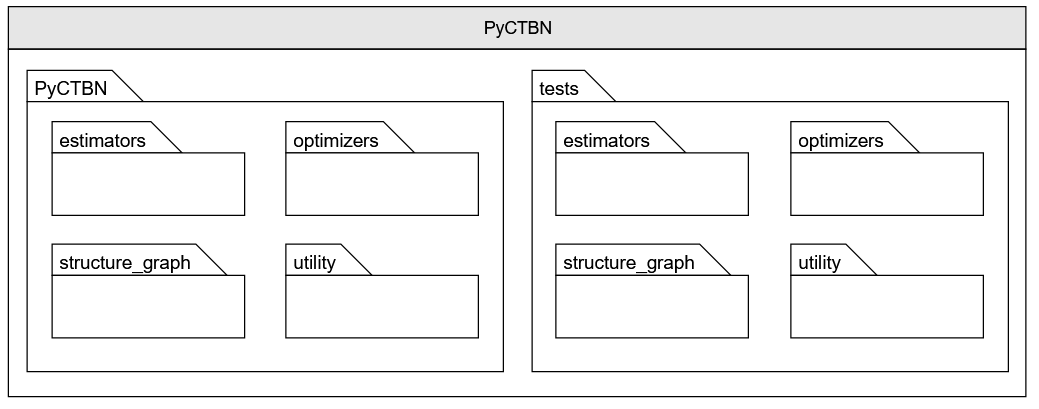
\includegraphics[width = 12cm]{packages}
    \centering
    \caption{Packages}
  \end{figure}

  La libreria PyCTBN è stata sviluppata basandosi sul paradigma \textit{OOP}, progettando un'adeguata
  organizzazione gerarchica delle classi, suddivise in \textbf{packages}.
  Analizzando la struttura delle directory che compongono il progetto partendo dal livello più alto, 
  la radice, viene effettuata una prima suddivisione in due package principali: \textit{PyCTBN} e
  \textit{tests}.\\
  Il package \textit{PyCTBN} contiene le classi effettive che implementano la logica applicativa,
  mentre \textit{tests} raggruppa le classi a cui è demandata la realizzazione di \textbf{Unit Test}.\\
  Al secondo livello, nel package \textit{PyCTBN} le classi sono state raggruppate in 4 packages, 
  in base alla funzione che svolgono:
  
  \begin{itemize}
    \item \textbf{structure\_graph}: Contiene tutte le classi dedicate alla modellazione della struttura completa di una
      CTBN in tutti i suoi aspetti. Alcuni esempi sono la classe \textit{NetworkGraph} (basata sulla libreria \textit{NetworkX}),
      che descrive la struttura del grafo orientato, la classe \textit{ConditionalIntensityMatrix}, che
      memorizza una singola CIM e quindi la classe \textit{SetOfCims} che si occupa di aggregare
      tutte le matrici associate ad uno specifico nodo in relazione ai valori dei nodi genitore.\\
      L'attività di stage si è focalizzata soprattutto sull'ampliamento di questo package, con
      l'introduzione delle classi \textit{TrajectoryGenerator} e \textit{NetworkGenerator}, spiegate nel
      dettaglio nella sezione dedicata.
      
    \item \textbf{estimators}: In questa cartella sono raccolte le classi deputate all'apprendimento,
      ovvero al calcolo della stima dei parametri (realizzato nella classe \textit{ParametersEstimator}) e della struttura di una CTBN
      (la cui implementazione si trova in \textit{StructureEstimator}, e nelle relative specializzazioni \textit{StructureConstraintBasedEstimator} e
      \textit{StructureScoreBasedEstimator}, in base all'algoritmo utilizzato).

    \item \textbf{optimizers}: Le tecniche di ottimizzazione di cui fanno uso gli stimatori trovano
      implementazione nelle classi appartenenti al package \textit{optimizers}. 
      Le strategie di ottimizzazione applicate in PyCTBN sono: \textit{HillClimbing} e \textit{TabuSearch} (per l'algoritmo di apprendimento Score-Based),
      e \textit{ConstraintBasedOptimizer} (per l'algoritmo di apprendimento Constraint-Based). 
      Tutte le classi relative all'ottimizzazione prevedono la realizzazione concreta dei metodi definiti nell'interfaccia \textit{Optimizer}.
    
    \item \textbf{utility}: Tutte le classi ausiliarie che si occupano di procedure di utilità,
      quali l'importazione e il pre-processing dei dati (\textit{AbstractImporter}, e la realizzazione
      \textit{JSONImporter} nel caso di dati in formato JSON) o l'esportazione (\textit{AbstractExporter} e quindi \textit{JSONExporter}).   
  \end{itemize}

  I test sono stati effettuati tramite il framework \textbf{unittest}, disponibile nel \textit{core}
  di Python. In particolare, a ciascuna classe in \textit{PyCTBN} è associata una corrispondente classe di test
  nel package \textit{tests}, che è perciò strutturato in modo simmetrico.

  \section{Diagramma delle Classi}
  Dopo aver presentato la struttura generale della libreria e l'organizzazione delle classi nei package,
  viene ora mostrato il diagramma delle classi in formato \textbf{UML} (Unified Modeling Language).\\
  Le classi il cui sviluppo è stato oggetto dello stage sono state rappresentate in grassetto all'interno del diagramma,
  allo scopo di metterne in evidenza la collocazione all'interno della libreria e la loro relazione con i 
  componenti già esistenti.
  Si tratta quindi di \textbf{TrajectoryGenerator} e \textbf{NetworkGenerator} per quanto riguarda
  il package \textit{structure\_graph}, e delle classi finalizzate all'esportazione delle reti,
  inserite in \textit{utility} (\textbf{AbstractExporter} e la relativa realizzazione \textbf{JSONExporter}).
    
  \begin{figure}[H]
    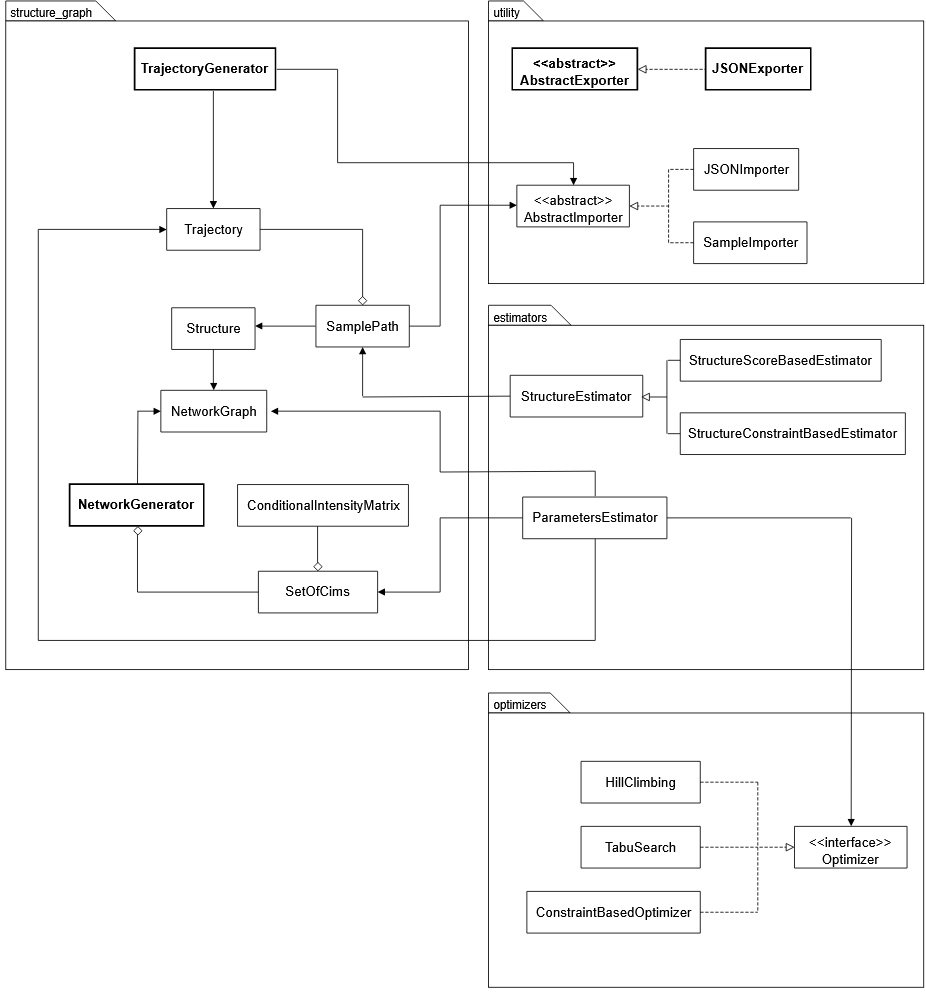
\includegraphics[width = \columnwidth]{dominio}
    \centering
    \caption{Diagramma di Dominio}
  \end{figure}

  \paragraph{}
  Il diagramma di dominio qui riportato omette i dettagli delle singole classi, quali attributi e metodi,
  limitandosi a descrivere le relazioni che intercorrono tra di esse e l'organizzazione generale della libreria.
  Verrà invece proposta nel seguito una descrizione esaustiva e dettagliata delle nuove classi aggiunte. 

  \newpage
  \section{Implementazioni}
  \paragraph{Naming}
  Al fine di preservare l'uniformità delle convenzioni stilistiche applicate al codice
  già esistente, per l'implementazione delle nuove classi sono state rispettate le seguenti regole,
  aderenti alle guidelines sul naming suggerite da Python:
  \begin{itemize}
    \item Notazione \textit{UpperCaseCamelCase} per le classi, e.g. \textit{TrajectoryGenerator}
    \item Notazione \textit{snake\_case} per i metodi, per le variabili e per gli attributi delle classi 
      (in questo caso preceduti da \textit{underscore}), capitalizzando tutte le lettere 
      costitutive di acronimi, e.g. \textit{\_network\_graph}, \textit{CTBN\_Sample()}
  \end{itemize}
  Nella firma dei metodi sviluppati sono stati specificati i \textit{tipi} dei parametri richiesti,
  garantendo maggiore leggibilità e chiarezza. Si è scelto inoltre di prediligere
  l'utilizzo di named arguments (\textit{keywords}) nell'ambito dell'invocazione
  di metodi, ottenendo maggiore flessibilità e favorendo la comprensione del significato
  degli argomenti.\\
  Si è cercato ovviamente di scegliere nomi significativi per variabili e metodi
  in relazione alla semantica del ruolo che ricoprono, rendendoli il più possibile
  autoesplicativi. 

  \paragraph{}
  Vengono ora descritte le implementazioni delle nuove classi introdotte in PyCTBN,
  vagliando le scelte architetturali adottate, le strutture dati progettate e
  l'integrazione con le altre funzionalità della libreria.\\
  Questa sezione ha inoltre lo scopo di documentare i metodi, analizzandone i parametri
  in ingresso e i valori restituiti, riportando anche snippets di codice al fine di mostrarne
  esempi concreti di utilizzo.  
  
  \subsection{TrajectoryGenerator}
  \paragraph{}
  È questa la classe che costituisce il fulcro del lavoro svolto e della presente trattazione.
  \textbf{TrajectoryGenerator} include infatti la realizzazione del metodo 
  \textit{CTBN\_Sample}, il cui pseudo-codice è stato discusso nel capitolo 2.2.
  
  \begin{figure}[H]
    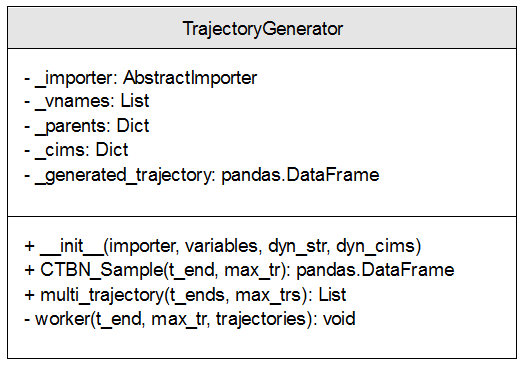
\includegraphics[width = 8cm]{trajectory_generator}
    \centering
    \caption{Classe TrajectoryGenerator}
    \label{fig:trajectory_generator}
  \end{figure}

  Come si può notare dal diagramma di classe riportato in Figura \ref{fig:trajectory_generator}, il costruttore (metodo \textit{\_\_init\_\_})
  accetta 4 parametri, ma l'utilizzo del primo è mutualmente esclusivo rispetto ai successivi. Ciò significa 
  che le informazioni riguardanti la rete su cui generare la traiettoria possono essere estratte dall'\textit{AbstractImporter}
  al primo parametro se questo è definito, o in alternativa passate singolarmente in corrispondenza di \textit{variables} (le variabili),
  \textit{dyn\_str} (gli archi del grafo) e \textit{dyn\_cims} (le CIM).
  
  \paragraph{}
  Poiché il campionamento di una traiettoria impiega intensivamente le informazioni riguardanti
  la struttura della rete (il grafo) e le CIM, risulta cruciale ai fini della velocità di esecuzione
  fare in modo che l'accesso a tali dati avvenga nel minor tempo possibile.\\
  Per questo motivo, il costruttore della classe si occupa di eseguire una procedura di \textit{pre-processing} 
  sui parametri in ingresso, al fine di costruire delle strutture dati ottimizzate in relazione alle operazioni che verranno eseguite.\\
  Per chiarire questo concetto, si assuma di voler generare una traiettoria sulla rete rappresentata
  nella struttura dati dell'Esempio 3.2.1. In questo caso quindi, gli archi fra i nodi
  sarebbero memorizzati tramite il seguente \textit{pandas.DataFrame}:
  
  \begin{center}
    \begin{tabular}{lll}
      \toprule
      {} & From & To \\   
      \midrule
      0 & X & Z \\  
      1 & Y & X \\  
      2 & Z & X \\    
      \bottomrule
    \end{tabular} 
  \end{center} 

  In questo formato non risulta però immediato ottenere l'elenco dei genitori di un certo nodo, informazione
  frequentemente necessaria per determinare le dipendenze di una variabile e prelevare di conseguenza i coefficienti dalle CIM.
  Per tale ragione si è deciso di associare all'attributo \textit{\_parents} un \textbf{dict} di Python (ovvero una Hashmap), che
  permette di accedere al valore associato ad una specifica chiave in tempo costante \textit{O(1)} nel caso generale, strutturato
  come segue:

  \begin{lstlisting}[language=json]
    {
      "X": ["Y", "Z"], 
      "Y": [], 
      "Z": ["X"]
    }
  \end{lstlisting}

  Basandosi su considerazioni analoghe vengono valorizzati gli altri attributi della classe.
  In particolare, \textit{\_vnames} si riferisce ad una \textbf{list} contenente le labels delle variabili della rete, 
  mentre \textit{\_cims} è un \textbf{dict} in cui a ciascuna chiave (label della variabile) è associata un'istanza della classe \textit{SetOfCims}, 
  che si occupa di gestire tutte le CIM associate a tale variabile.

  \paragraph{CTBN\_Sample}
  Questo metodo si occupa della generazione effettiva di una \textbf{singola} traiettoria, e riflette
  fedelmente lo pseudo-codice introdotto in precedenza. Oltre alla condizione standard di terminazione
  basata sul raggiungimento di un tempo massimo $t_{end}$, è stato ritenuto opportuno prevedere
  un'alternativa tale per cui l'evoluzione dello stato della rete, e quindi la creazione della traiettoria,
  si interrompe quando viene raggiunto un numero $n_{tr}$ di campioni generati.\\
  Questa premessa consente di dedurre la semantica dei parametri richiesti dal metodo, ovvero \textit{t\_end}
  e \textit{max\_tr}, che determinano quindi rispettivamente il tempo massimo raggiungibile durante 
  il campionamento e il numero di transizioni di interesse. L'implementazione non prevede un utilizzo
  congiunto dei due argomenti, infatti \textit{max\_tr} viene ignorato se \textit{t\_end} è diverso da -1
  (che è il valore di default per entrambi).\\ 
  È utile sottolineare come non sia possibile conoscere a priori, prima dell'esecuzione, il numero
  di campioni di cui sarà composta la traiettoria nel caso in cui venga stabilito il tempo massimo
  come condizione di terminazione. Viceversa, tale valore è ovviamente noto, in quanto viene imposto, 
  se si utilizza la variante che fa uso del numero di transizioni consentite.\\
  Un'ulteriore dissomiglianza rispetto allo pseudo-codice commentato, consiste nel valore iniziale attribuito
  alle variabili all'istante $t = 0$: è stato infatti ritenuto ininfluente assegnare a tutte le variabili
  il valore 0 piuttosto che determinarlo dalla distribuzione iniziale.\\
  Per la generazione casuale dell'intervallo di tempo $\Delta t$ dopo il quale avverrà la prossima 
  transizione, è stato sfruttato il metodo \textbf{random.exponential}, messo a disposizione da \textit{numpy}.
  A questo metodo deve essere passato un parametro $\beta = \frac{1}{\lambda}$, di tipo \textit{float}
  e non negativo. L'argomento, come ampiamente discusso, consiste nel valore della CIM che si trova 
  sulla diagonale, alla riga corrispondente allo stato attuale della variabile. Per soddisfare la condizione di non-negatività 
  imposta dal metodo, viene utilizzato l'opposto del coefficiente della CIM, dal momento che quest'ultimo è ovviamente negativo.\\
  Quando viene raggiunto il tempo $t$ in cui avviene la transizione di una variabile $X$, è necessario determinare
  il nuovo valore che essa deve assumere. Innanzitutto viene quindi prelevata la CIM
  da utilizzare in relazione allo stato attuale dei genitori della variabile che effettua la transizione.
  Questo è facilmente attuato tramite il metodo \textit{filter\_cims\_with\_mask} della classe \textit{SetOfCims}
  che, presa in ingresso una lista composta dai valori dei genitori, restituisce la matrice corrispondente.
  Se $X = x$, viene isolata la \textit{x-esima} riga della CIM stabilita, ovvero quella relativa alle
  probabilità istantanee di lasciare lo stato $x$, e si procede come segue:

  \begin{itemize}
    \item Si assegna il valore 0 all'\textit{x-esimo} elemento della riga in questione
    \item Si normalizza la riga per fare in modo che la somma dei suoi elementi sia 1
  \end{itemize}

  L'array così ottenuto viene perciò utilizzato come argomento del metodo \textbf{random.multinomial}
  (anche in questo caso fornito da \textit{numpy}), allo scopo di estrarre casualmente dalla distribuzione multinomiale
  il nuovo valore che verrà assegnato ad $X$.\\
  Per chiarire quanto esposto, si procede con un esempio riguardante l'estrazione dei coefficienti dalla CIM.

  \begin{exmp}[Estrazione dei coefficienti dalla CIM]
    Sia $X$ una variabile il cui nodo associato non possiede archi entranti, ovvero priva di dipendenze.
    Si supponga che $X = 1$ all'istante corrente.\\
    L'unica CIM di $X$ è la matrice riportata di seguito:

    \[
      \begin{bmatrix}
        -1.9695 & 0.3461 & 1.6234\\
        0.7465 & -1.3067 & 0.5602\\
        0.8775 & 1.4581 & -2.3356
      \end{bmatrix} 
    \]

    Per quanto riguarda l'estrazione casuale di $\Delta t$ dalla distribuzione esponenziale,
    il parametro utilizzato sarà $\lvert -1.3067 \lvert \; = \; 1.3067$, poiché è l'elemento in posizione (1, 1).\\
    Nell'ambito della transizione, invece, verrà prima estratta la riga associata allo stato 1:
  
    \[
      \begin{bmatrix}
        0.7465 & -1.3067 & 0.5602
      \end{bmatrix} 
    \]

    Posto a 0 l'elemento diagonale:

    \[
      \begin{bmatrix}
        0.7465 & 0 & 0.5602
      \end{bmatrix} 
    \]

    E infine normalizzata in modo che i suoi valori rappresentino probabilità effettive:

    \[
      \begin{bmatrix}
        0.5713 & 0 & 0.4287
      \end{bmatrix} 
    \]

    Questo array, la cui somma degli elementi è pari ad 1, sarà quindi il parametro di
    \textbf{numpy.random.multinomial}.
  \end{exmp}

  \paragraph{}
  La traiettoria generata viene memorizzata in un oggetto di tipo \textbf{DataFrame} di \textit{pandas},
  aggiungendo ad esso una riga ogni volta che avviene una transizione e una variabile cambia stato.
  Allo scopo di rispettare la convenzione enunciata nel Capitolo 3.2, come ultimo elemento della traiettoria
  viene aggiunta una riga in cui tutte le variabili hanno valore -1.
  Questo oggetto rappresenta il valore di ritorno di \textit{CTBN\_Sample}.
  Viene ora mostrato un esempio di esecuzione, includendo una parte della traiettoria generata.

  \begin{exmp}
    Si supponga di voler generare una traiettoria costituita da 1000 osservazioni sulla CTBN basata sul grafo riportato in Figura 3.1,
    e che la struttura di tale rete sia memorizzata nel file \emph{example.json}.\\
    Il seguente frammento di codice mostra un esempio di utilizzo di \emph{TrajectoryGenerator} per tale
    scopo.
  \end{exmp}

  \begin{lstlisting}[language=python]
    j1 = JsonImporter(
      file_path = "example.json", 
      samples_label = "samples",
      structure_label = "dyn.str", 
      variables_label = "variables",
      time_key = "Time",
      variables_key = "Name"
    )
    
    j1.import_data(0)

    tg = TrajectoryGenerator(importer = j1)
    sigma = tg.CTBN_Sample(max_tr = 1000)
  \end{lstlisting}

  \textit{La traiettoria prodotta, contenuta in \emph{sigma}, sarà nella seguente forma:}

  \[
    \begin{tabular}{lllll}
      \toprule
      {} &     Time &   X &   Y &   Z \\
      \midrule
      0    &        0 &   0 &   0 &   0 \\
      1    &   0.0494 &   2 &   0 &   0 \\
      2    &   1.5477 &   2 &   1 &   0 \\
      3    &   1.692 &   2 &   1 &   2 \\
      4    &   1.7851 &   1 &   1 &   2 \\
      5    &   1.9497 &   2 &   1 &   2 \\
      6    &   2.2106 &   2 &   2 &   2 \\
      7    &   2.3166 &   2 &   2 &   1 \\
      8    &   2.3999 &   2 &   0 &   1 \\
      9    &   2.553 &   2 &   0 &   0 \\
      10   &   2.8792 &   2 &   0 &   2 \\  
      \vdots  &   \vdots    & \vdots & \vdots & \vdots \\
      990  &   595.85 &   2 &   0 &   1 \\
      991  &   596.89 &   2 &   0 &   0 \\
      992  &  596.943 &   2 &   2 &   0 \\
      993  &   597.96 &   2 &   1 &   0 \\
      994  &  598.155 &   0 &   1 &   0 \\
      995  &  598.696 &   0 &   0 &   0 \\
      996  &  598.856 &   0 &   0 &   2 \\
      997  &  599.426 &   0 &   2 &   2 \\
      998  &   599.58 &   1 &   2 &   2 \\
      999  &  601.761 &   2 &   2 &   2 \\
      1000 &  602.012 &  -1 &  -1 &  -1 \\
      \bottomrule
    \end{tabular}
  \]

  \subsubsection{Multiprocessing}
  Nel contesto dell'utilizzo reale della libreria, raramente viene generata una singola traiettoria, ma si usa piuttosto
  campionarne diverse che vengono poi aggregate. Un primo approccio potrebbe prevedere di generare
  \textit{sequenzialmente} le traiettorie, iniziandone una solo dopo che la precedente è stata completata.
  La possibilità di ottimizzazione e velocizzazione di questo metodo, tuttavia, è suggerita dal fatto
  che ciascuna traiettoria è completamente indipendente dalle altre, e la sua generazione non dipende
  dalle traiettorie campionate in precedenza, favorendo quindi un'implementazione basata sull'esecuzione in parallelo.\\
  Per realizzare la parallelizzazione della procedura, si è deciso di basarsi sul \textbf{multi-processing},
  scartando il \textbf{multi-threading}, a causa delle problematiche che Python comporta
  nell'utilizzo dei Thread, legate soprattuto alla gestione attuata dal \textbf{GIL} (Global Interpreter Lock).
  Tale componente infatti, oltre ad una gestione non ottimale della memoria, permette l'esecuzione di un solo thread alla volta, 
  ostacolando un concreto miglioramento delle prestazioni.\\
  Il multi-processing, invece, permette di eludere le restrizioni imposte dal GIL dal momento che
  ad ogni processo viene assegnato un distinto interprete e uno spazio di memoria dedicato, favorendo
  un reale parallelismo. Le classi e i metodi necessari sono contenuti nel package \textbf{multiprocessing},
  disponibile nel core di Python.\\
  La generazione di più traiettorie contemporaneamente è attuabile tramite il metodo
  \textit{multi\_trajectory}, i cui parametri hanno la stessa semantica di quelli di \textit{CTBN\_Sample},
  trattandosi sostanzialmente di un metodo wrapper. 
  Di conseguenza, i parametri \textit{t\_ends} e \textit{max\_trs} sono due \textbf{List} e contengono rispettivamente
  l'elenco dei tempi massimi e del numero di transizioni delle traiettorie da generare.
  Non è possibile utilizzarli congiuntamente, il secondo parametro viene infatti preso in considerazione
  solo se il primo non è definito. Il numero di traiettorie che verranno campionate è quindi una conseguenza del numero 
  di elementi presenti nella lista passata come parametro.\\
  Vengono dunque inizializzati tanti processi quante sono le traiettorie da generare, tramite
  la classe \textbf{multiprocessing.Process}, e i pandas.DataFrame prodotti da ciascun processo vengono
  salvati in una lista condivisa che le aggrega.\\
  La procedura target che viene eseguita da ciascun processo è definita nel metodo \textit{worker},
  che si occupa semplicemente di generare una singola traiettoria e di aggiungerla alla lista
  condivisa.\\
  Dopo aver avviato (tramite il metodo \textit{Process.start()}) i processi creati, \textit{multi\_trajectory}
  attende che tutti terminino la loro esecuzione (attraverso \textit{Process.join()}), prima di ritornare al chiamante
  la lista contenente le traiettorie prodotte.

  \begin{exmp}
    Si vogliono generare in parallelo 3 traiettorie i cui tempi massimi sono 100, 200 e 500.
    Si supponga che la struttura della rete sia già stata importata (come mostrato nell'esempio
    precedente) e sia contenuta nell'oggetto \emph{j1:JsonImporter}.\\
    Il seguente frammento di codice mostra un esempio di utilizzo di \emph{TrajectoryGenerator} per tale
    scopo.
  \end{exmp}

  \begin{lstlisting}[language=python]
    tg = TrajectoryGenerator(importer = j1)
    trajectories = tg.multi_trajectory(
      t_ends = [100, 200, 500]
    )
  \end{lstlisting}

  \begin{figure}[H]
    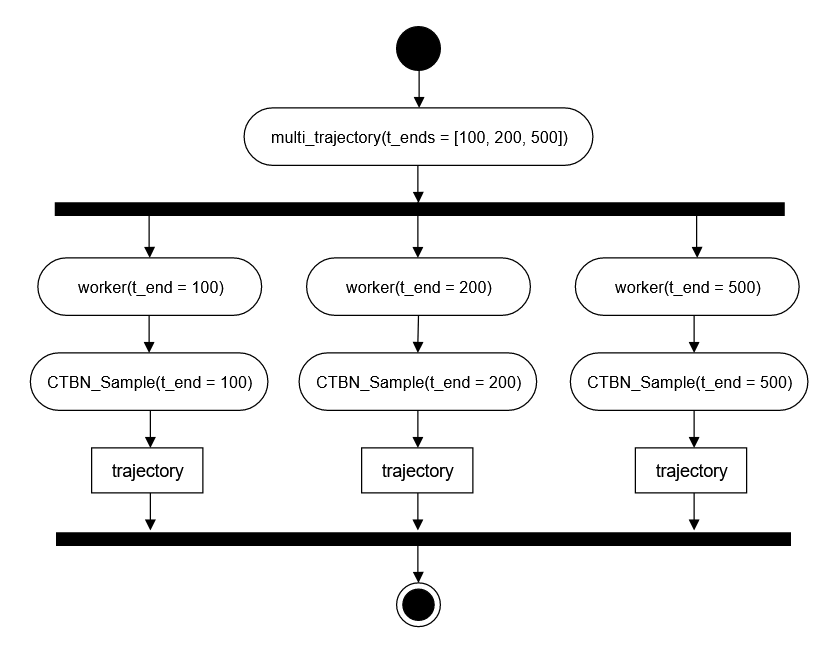
\includegraphics[width = \columnwidth]{activity}
    \centering
    \caption{Diagramma di Attività - multi\_trajectory}
  \end{figure}

  \paragraph{}
  Nel Capitolo 4.7 verrà mostrato un confronto tra le prestazioni ottenute tramite l'utilizzo del multi-processing e quelle dell'esecuzione sequenziale,
  volto a mettere in risalto i miglioramenti ottenuti.

  \subsection{NetworkGenerator}
  \textbf{NetworkGenerator} espone un insieme di metodi finalizzati alla generazione randomica di una rete.
  In particolare, questa classe permette di produrre il grafo e le CIM conoscendo a priori il numero di variabili (correlate dalla relativa cardinalità), 
  specificate nell'input.
  
  \begin{figure}[H]
    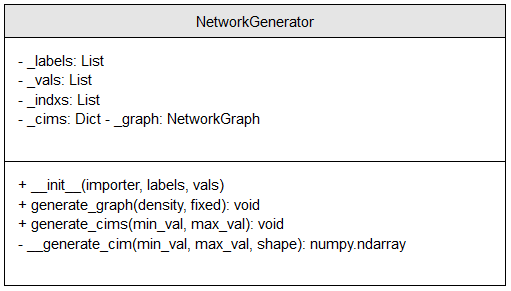
\includegraphics[width = 8cm]{network_generator}
    \centering
    \caption{Classe NetworkGenerator}
  \end{figure}

  Il costrutture della classe, infatti, accetta due \textbf{List} come parametri: \textit{labels} e \textit{vals}.
  Il primo è l'elenco delle etichette associate alle variabili che costituiranno la CTBN generata, 
  le cui cardinalità sono definite nel secondo parametro (nella posizione omologa). 
  Il metodo \textit{\_\_init\_\_} si limita ad assegnare tali parametri ai corrispondenti attributi 
  di classe e ad inizializzare \textit{\_indxs} (che non è altro che un'enumerazione in ordine crescente
  di lunghezza pari al numero di variabili).\\
  La costruzione del grafo e la generazione delle CIM vengono gestite, nell'ordine, dal metodo \textit{generate\_graph} e 
  dal metodo \textit{generate\_cims}, le cui modalità di implementazione vengono illustrate nelle
  relative descrizioni che seguono.

  \paragraph{generate\_graph}
  Si occupa della generazione di un grafo orientato, basandosi sull'idea di stabilire, per ciascuna coppia di variabili $(X, Y)$
  se esiste un arco da $X$ a $Y$ e viceversa. La presenza di un arco è determinata concettualmente tramite
  il cosiddetto ``lancio di una moneta'', ovvero estraendo casualmente un valore da una distribuzione \textbf{Bernoulliana},
  stabilendo la convenzione tale per cui l'esistenza dell'arco corrisponde al valore estratto 1.\\
  Una variabile aleatoria distribuita secondo una Bernoulliana di parametro $p$, infatti, può assumere
  solo i valori 0 e 1 rispettivamente con probabilità $(1 - p)$ e $p$. Il valore di $p$ è definito dal parametro
  \textit{density} di \textit{generate\_graph}, volto appunto a calibrare la densità del grafo.\\
  Anche in questo caso, l'estrazione randomica del numero è stata realizzata sfruttando \textit{numpy},
  e in particolare il metodo \textbf{random.binomial}. Poiché una variabile distribuita secondo una
  binomiale è definita come la somma di $n$ variabili Bernoulliane di uguale parametro $p$,
  tale metodo è stato usato ponendo il parametro $n$ a 1.\\
  Il nucleo di \textit{generate\_graph}, sintetizzando, consiste nella seguente \textbf{list comprehension}:

  \begin{lstlisting}[language=python]
    edges = [(i, j) for i in self._labels 
      for j in self._labels 
      if np.random.binomial(1, density) == 1 and i != j]
  \end{lstlisting}

  Il parametro $density$, tuttavia, rappresenta una probabilità e non garantisce che la
  densità della rete generata sia effettivamente pari al valore richiesto. Per questa 
  ragione è stato introdotto il parametro booleano $fixed$, che se impostato a \textit{true}
  determina una diversa procedura di generazione degli archi, assicurando che la densità
  del grafo prodotto corrisponda realmente a $density$. Questa procedura alternativa
  consiste nel creare una lista contenente tutti gli archi possibili (eccetto i cappi),
  ordinarla casualmente, ed estrarre i primi $e$ elementi (il numero di archi $e$ è ottenuto 
  dalla formula inversa ricavabile dall'equazione \eqref{eq:density} relativa alla densità).
  Se la densità richiesta dovesse implicare un numero di archi non intero, verrebbe sollevata un'eccezione
  di tipo \textit{RuntimeError}.

  \paragraph{generate\_cims}
  Poiché il numero di CIM che devono essere generate per ciascuna variabile è una diretta conseguenza della struttura della rete
  (dato che le matrici devono rispecchiare le dipendenze tra le variabili) il metodo \textit{generate\_cims} deve obbligatoriamente 
  essere eseguito dopo \textit{generate\_graph}, in modo tale che il grafo sia definito.\\
  I parametri \textit{min\_val} e \textit{max\_val} consentono di stabilire il range numerico all'interno del quale
  si devono trovare i coefficienti delle matrici.\\
  Il metodo \textit{generate\_cims} si occupa esclusivamente di enumerare, per ciascun nodo della rete, le possibili combinazioni
  degli stati dei genitori, associando a ciascuna di esse una CIM.\\
  Al fine di scomporre la procedura in sottoproblemi di dimensioni minori, la generazione effettiva di una singola CIM senza contesto
  (vale a dire a prescindere dalla struttura della rete) è demandata al metodo privato \textit{\_\_generate\_cim}.
  Il parametro \textit{shape} di quest'ultimo metodo fornisce informazioni sulle dimensioni della matrice che
  deve essere generata (il numero di righe e di colonne è chiaramente uguale), e corrisponde quindi
  alla cardinalità della variabile a cui verrà assegnata la CIM prodotta.\\
  Il processo di costruzione di una CIM prevede di determinare preliminarmente gli elementi che si trovano 
  sulla diagonale maggiore, estraendoli da una distribuzione \textbf{uniforme}, e successivamente di calcolare
  gli altri coefficienti delle righe di conseguenza (quindi facendo in modo che la loro somma corrisponda all'opposto
  del valore dell'elemento diagonale). Per fare ciò, si determinano casualmente i coefficienti che compongono
  le righe (sempre utilizzando una distribuzione uniforme), si normalizzano affinché la loro somma sia 1 e infine
  si moltiplicano per il valore assegnato all'elemento diagonale.\\
  L'estrazione di valori casuali dalla distribuzione uniforme è delegata a \textbf{numpy.random.rand}.
  Si è convenzionalmente deciso di arrotondare tutti i coefficienti a 4 cifre decimali.

  \paragraph{Proprietà di Faithfulness}
  Nella procedura di generazione delle CIM è stata ignorata la possibilità che le matrici prodotte non
  rispecchino la realtà.\\
  La proprietà di \textbf{faithfulness} di una rete statuisce che le CIM devono implicitamente esprimere le dipendenze tra le variabili.
  Esemplificando il concetto, se una variabile $X$ dipende da una variabile $Y$, al variare di $Y$ devono variare le matrici di $X$.
  Per assurdo, se le CIM restassero uguali al variare di $Y$, si potrebbe desumere che i nodi sono indipendenti.\\ 
  La tecnica fondata sull'estrazione casuale dei coefficienti che è stata adottata nell'implementazione, tuttavia, non esclude che 
  possano essere prodotte matrici molto simili, nel caso limite uguali, violando tale proprietà.

  \subsection{AbstractExporter}
  \paragraph{}
  Poiché PyCTBN non forniva strumenti per l'esportazione e il salvataggio su file delle strutture
  e delle traiettorie, è stato ritenuto opportuno sviluppare una gerarchia di classi finalizzata
  a soddisfare queste necessità. L'utilizzo dei file è stato particolarmente importante anche per
  facilitare la comunicazione e lo scambio dei dati tra i vari componenti della libreria,
  sfruttando le procedure già esistenti di pre-processing dei dataset.

  \begin{figure}[H]
    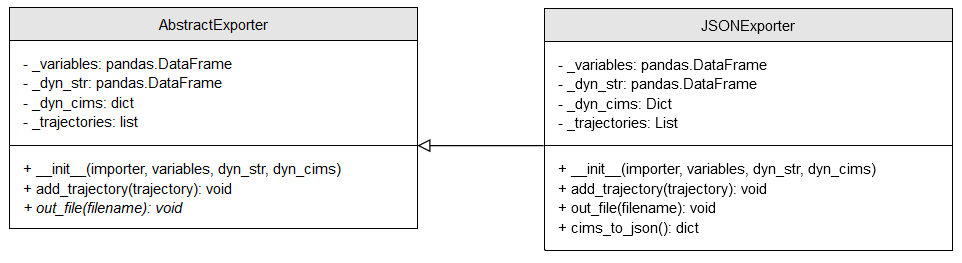
\includegraphics[width = \columnwidth]{exporter}
    \centering
    \caption{Classe AbstractExporter - JSONExporter}
  \end{figure}

  Per avvalorare l'estensibilità della libreria e non precludere la possibilità di utilizzare formati 
  diversi dal JSON, le scelte progettuali relative all'esportazione sono state mirate a creare
  una simmetria con la struttura delle classi previste per le fasi di importazione.
  Come accennato, infatti, il package utility include una classe astratta \textit{AbstractImporter}
  che definisce le funzionalità generiche di importazione e pre-processing dei dati, che trovano poi
  realizzazione nelle diverse specializzazioni legate ai vari formati, come ad esempio \textit{JSONImporter}.
  Questa organizzazione gerarchica rende agevole slegarsi dal formato JSON, adottando ad esempio il formato \textit{csv}, 
  senza ripercussioni sull'interazione con le altre classi della libreria.\\
  A prescindere dal formato in cui verrà esportata la rete, quindi, \textit{AbstractExporter}
  raggruppa tutti i dati che la descrivono (che corrispondono sostanzialmente ai campi dell'oggetto JSON illustrato
  nel Capitolo 3.2), tramite le strutture dati utilizzate all'interno della libreria.
  I campi di \textit{AbstractExporter} saranno perciò organizzati come segue:

  \begin{itemize}
    \item \_variables: istanza di \textit{pandas.DataFrame} contenente, per ciascuna variabile della rete,
      l'etichetta associata e la cardinalità
    \item \_dyn\_str: istanza di \textit{pandas.DataFrame} in cui ogni riga rappresenta un arco del grafo,
      nel formato mostrato nel Capitolo 3.5.1
    \item \_dyn\_cims: hashmap in cui le chiavi sono le etichette delle variabili, e a ciascuna chiave è 
      assegnato l'oggetto di classe \textit{SetOfCims} corrispondente
    \item \_trajectories: lista contenente le traiettorie (memorizzate come istanze di \textit{pandas.DataFrame})
  \end{itemize}

  \paragraph{}
  Il campo \textit{\_trajectories} viene inizializzato come lista vuota, e le traiettorie possono essere
  successivamente aggiunte tramite il metodo \textit{add\_trajectory}.\\
  Una volta che tutti i dati riguardanti la rete sono stati forniti alla classe \textit{AbstractExporter},
  il file di output può essere creato tramite il metodo \textit{out\_file}, che accetta come
  unico parametro il \textit{filename}. Le operazioni eseguite da tale metodo, oltre che l'estensione del file,
  dipendono ovviamente dalla specializzazione di \textit{AbstractExporter} che è stata istanziata.

  \paragraph{}
  La classe \textit{JSONExporter} include un metodo aggiuntivo, \textit{cims\_to\_json}, 
  che si occupa di ristrutturare gli oggetti di tipo \textit{SetOfCims} convertendoli in un formato
  adeguato all'esportazione in \textit{JSON}.

  \section{Diagramma di Sequenza}
  Il diagramma in Figura 4.8 mostra un possibile scenario di interazione fra le nuove classi sviluppate,
  mettendo in risalto l'ordine, la successione temporale, in cui ciascuna operazione viene eseguita.\\
  Tale esempio inclue la generazione di una rete, invocando prima \textit{generate\_graph} e solo successivamente
  \textit{generate\_cims}. Le componenti della rete creata vengono usate per inizializzare un oggetto di tipo
  \textit{JSONExporter} e un oggetto di classe \textit{TrajectoryGenerator}, dopodiché si generano iterativamente
  delle traiettorie che vengono man mano aggiunte all'exporter tramite \textit{add\_trajectory}. 
  Infine viene scritto il file in output.

  \begin{figure}[H]
    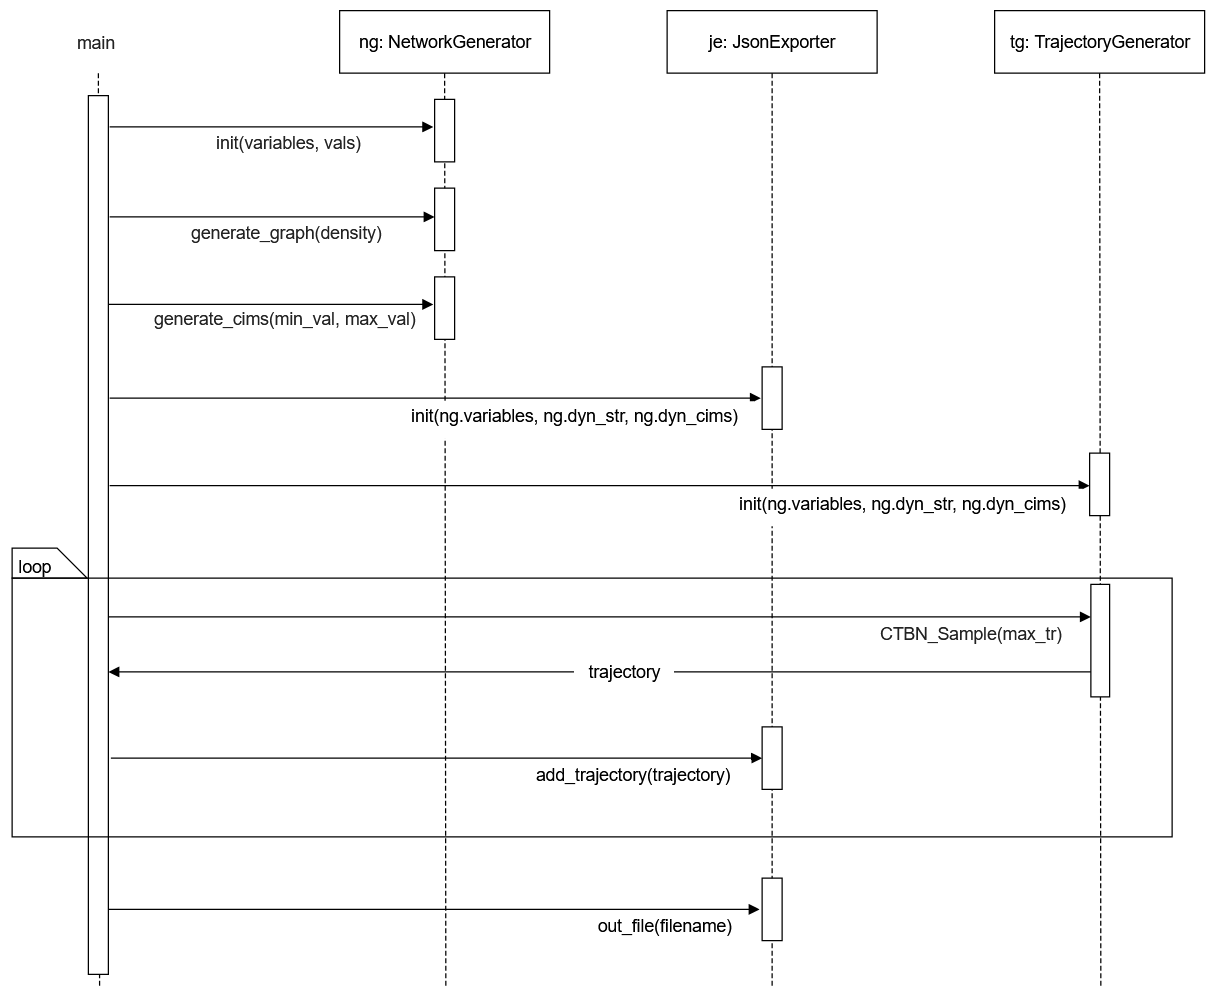
\includegraphics[width = \columnwidth]{sequenza}
    \centering
    \caption{Diagramma di Sequenza}
  \end{figure}

  \section{Analisi delle Prestazioni}
  \paragraph{}
  Uno dei principali parametri di valutazione di PyCTBN è l'efficienza, e perché la libreria sia
  fruibile è importante che i tempi di esecuzione non diventino eccessivamente proibitivi al 
  crescere delle dimensioni delle reti.
  Questo capitolo, quindi, si occupa di analizzare i risultati ottenuti con le implementazioni
  di PyCTBN, sia in relazione ai tempi di esecuzione che alla quantità di memoria RAM occupata,
  in particolare per quanto riguarda le procedure più critiche, ovvero la generazione delle reti
  e il campionamento delle traiettorie, focalizzandosi altresì sui benefici ottenuti dall'implementazione
  parallela.

  \subsection{Parametri considerati}
  Poiché le prestazioni dei metodi dipendono dalla struttura della rete, le misurazioni sono state
  effettuate per ciascuna combinazione ottenuta al variare dei seguenti parametri:
  \begin{itemize}
    \item numero di variabili (5, 10, 15 e 20)
    \item cardinalità delle variabili (binarie, ternarie e quaternarie)
    \item densità del grafo (0.1, 0.2, 0.3 e 0.4), resa effettiva tramite il parametro \textit{fixed}
      del metodo \textit{generate\_graph}
  \end{itemize}
  
  \paragraph{}
  Il tempo necessario per il campionamento di una traiettoria, piuttosto che quello
  richiesto per generare le CIM associate ad una rete, dipende non solo dalla densità
  del grafo, ma anche da come sono disposti gli archi. Una rete in cui tutti gli archi sono
  diretti verso un solo nodo, ad esempio, implica un numero maggiore di dipendenze e quindi tempi
  più elevati quando la variabile centrale compie una transizione.\\
  Per la misurazione delle prestazioni si è quindi deciso di prendere in considerazione, per
  ciascuna combinazione dei parametri scelti, i risultati prodotti da un insieme di 20 esecuzioni distinte.
  I valori mostrati sui grafici sono stati calcolati come \textbf{media} dei valori ottenuti, e per fornire informazioni
  sul comportamento delle osservazioni vengono riportate anche le relative \textbf{deviazioni standard}.\\
  I tempi di esecuzione sono espressi in secondi, mentre i valori relativi alla quantità di memoria
  RAM occupata sono da intendersi in MegaBytes.\\
  Per favorire la leggibilità e la comunicatività dei grafici, si è deciso di usare la scala logaritmica per l'asse
  delle ordinate.

  \paragraph{}
  Il tempo impiegato per l'esecuzione dipende logicamente dalla macchina su cui gli esperimenti
  vengono svolti, ma è ad ogni modo possibile trarre importanti informazioni considerando i valori
  in modo relativo, studiando l'andamento dei tempi al variare della complessità della rete.\\
  Per completezza di informazione, vengono comunque riportate le specifiche hardware più significative della macchina utilizzata:
  \begin{itemize}
    \item Processore Intel(R) Core(TM) i7-1065G7 CPU da 1.30GHz
    \item RAM 16GB
    \item SSD 512GB 
  \end{itemize}

  \subsection{TrajectoryGenerator}
  Per quanto concerne la classe \textit{TrajectoryGenerator}, la valutazione delle prestazioni
  è stata effettuata ovviamente sul metodo \textit{CTBN\_Sample}, in particolare generando traiettorie
  con un numero di transizioni prestabilito pari a 1000.

  \subsubsection{Tempi}
  \begin{figure}[H]
    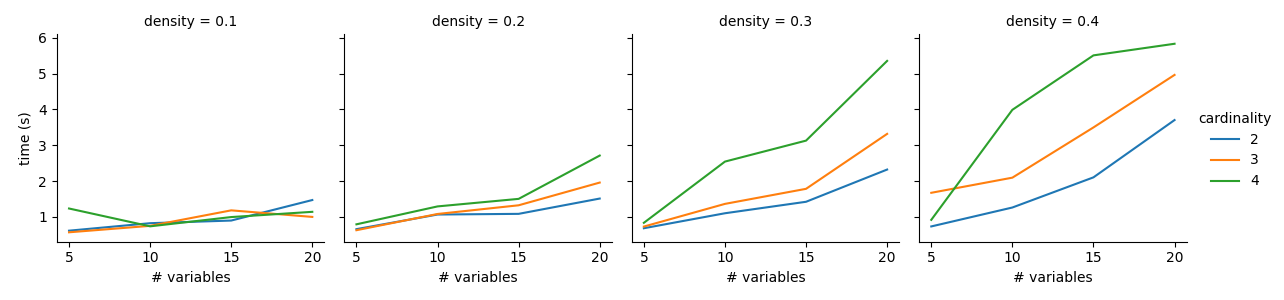
\includegraphics[width = \columnwidth]{times_trajectory}
    \centering
    \caption{Tempi di esecuzione - TrajectoryGenerator}
  \end{figure}

  \paragraph{}
  È possibile notare come il tempo necessario per il campionamento delle traiettorie sia molto
  prossimo allo zero nei casi in cui la rete abbia densità uguale a 0.1 o 0.2, a prescindere dal numero
  e dalla cardinalità delle variabili coinvolte. All'aumentare della complessità della rete, invece,
  il tempo impiegato cresce sensibilmente, in particolare nel caso di reti costituite da
  variabili quaternarie.\\
  Come testimoniato dai valori della deviazione standard sotto riportati, la variabilità dei tempi 
  è maggiore in reti più complesse, a dimostrazione del fatto che la distribuzione degli archi 
  all'interno del grafo influenza significativamente l'esecuzione. Le deviazioni standard più 
  elevate, infatti, sono state riscontrate in corrispondenza degli esperimenti su reti caratterizzate
  da densità più elevate.

  \vspace{6mm}

  \begin{center}
    \begin{tabular}{c|cc|cccc}
      \toprule
      $\# \; variables$ & {} & {} & $d = 0.1$ & $d = 0.2$ & $d = 0.3$ & $d = 0.4$\\
      \midrule
      \multirow{3}{*}{5} & \multirow{3}{*}{\rotatebox[origin=c]{90}{card.}} & 2 & 0.0428 & 0.4993 & 0.0530 & 0.0437\\
      {} & {} & 3 & 0.0415 & 0.0715 & 0.0831 & 1.3795\\
      {} & {} & 4 & 0.3656 & 0.6310 & 0.9214 & 1.3203\\

      \midrule
      \multirow{3}{*}{10} & \multirow{3}{*}{\rotatebox[origin=c]{90}{card.}} & 2 & 0.1060 & 0.1247 & 1.1147 & 0.3889\\
      {} & {} & 3 & 0.1055 & 0.8270 & 0.6428 & 3.5571\\
      {} & {} & 4 & 0.1496 & 1.0902 & 13.6267 & 71.7103\\

      \midrule
      \multirow{3}{*}{15} & \multirow{3}{*}{\rotatebox[origin=c]{90}{card.}} & 2 & 0.0570 & 0.0885 & 0.4706 & 1.9183\\
      {} & {} & 3 & 0.1153 & 4.3084 & 20.7983 & 85.2990\\
      {} & {} & 4 & 0.0365 & 3.2622 & 18.4352 & 98.1215\\

      \midrule
      \multirow{3}{*}{20} & \multirow{3}{*}{\rotatebox[origin=c]{90}{card.}} & 2 & 1.8115 & 0.3210 & 4.0379 & 15.4693\\
      {} & {} & 3 & 0.1187 & 0.3121 & 2.3850 & 25.3890\\
      {} & {} & 4 & 0.7821 & 11.1102 & 65.2257 & 152.0916\\
      \bottomrule
    \end{tabular}
    
    \captionof{table}{Dev. Standard dei tempi di esecuzione - TrajectoryGenerator}
  \end{center}

  \vspace{6mm}

  \subsubsection{Memoria}
  \paragraph{}
  Come si può notare dai grafici, anche l'utilizzo di memoria cresce in modo esponenziale in
  corrispondenza di reti più grandi e più dense. Questo comportamento è motivato innanzitutto dalla dimensione del 
  \textit{DataFrame} contenente la traiettoria, che sarà costituito da un numero di colonne pari al numero
  di variabili che costituiscono la rete. In aggiunta, anche il numero di \textit{Conditional Intensity Matrices} coinvolte, 
  e la dimensione di ciascuna matrice, dipendono rispettivamente dalla densità del grafo e dalla 
  cardinalità delle variabili.\\
  Dall'analisi dei dati relativi alle deviazioni standard, invece, è possibile estrarre informazioni
  significative riguardo alla quantità di spazio richiesta per la generazione di una traiettoria.
  Ad eccezione dei valori dell'indice calcolati sui risultati delle misurazioni provenienti da reti molto grandi, infatti, 
  tutti i valori sono prossimi allo zero, suggerendo un'occupazione di memoria pressoché costante a
  parità di parametri utilizzati.

  \begin{figure}[H]
    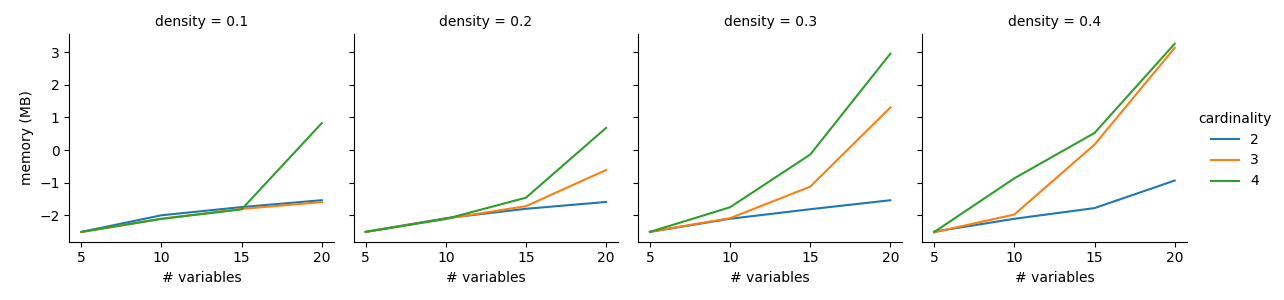
\includegraphics[width = \columnwidth]{memory_trajectory}
    \centering
    \caption{Utilizzo della memoria - TrajectoryGenerator}
  \end{figure}

  \vspace{10mm}

  \begin{center}
    \begin{tabular}{c|cc|cccc}
      \toprule
      $\# \; variables$ & {} & {} & $d = 0.1$ & $d = 0.2$ & $d = 0.3$ & $d = 0.4$\\
      \midrule
      \multirow{3}{*}{5} & \multirow{3}{*}{\rotatebox[origin=c]{90}{card.}} & 2 & 0.0003 & 0.0051 & 0.0001 & 0.0005\\
      {} & {} & 3 & 0.0003 & 0.0005 & 0.0001 & 0.0001\\
      {} & {} & 4 & 0.0002 & 0.0003 & 0.0035 & 0.0032\\

      \midrule
      \multirow{3}{*}{10} & \multirow{3}{*}{\rotatebox[origin=c]{90}{card.}} & 2 & 0.0570 & 0.0103 & 0.0001 & 0.0002\\
      {} & {} & 3 & 0.0007 & 0.0002 & 0.0101 & 0.0002\\
      {} & {} & 4 & 0.0002 & 0.0025 & 0.1249 & 0.5664\\

      \midrule
      \multirow{3}{*}{15} & \multirow{3}{*}{\rotatebox[origin=c]{90}{card.}} & 2 & 0.0485 & 0.0116 & 0.0029 & 0.0089\\
      {} & {} & 3 & 0.0099 & 0.0509 & 0.2461 & 0.9912\\
      {} & {} & 4 & 0.0005 & 0.1226 & 0.0003 & 1.0029\\

      \midrule
      \multirow{3}{*}{20} & \multirow{3}{*}{\rotatebox[origin=c]{90}{card.}} & 2 & 0.0438 & 0.0076 & 0.0437 & 0.2317\\
      {} & {} & 3 & 0.0043 & 0.3434 & 3.3019 & 27.7697\\
      {} & {} & 4 & 0.1768 & 3.4122 & 16.9224 & 24.8423\\
      \bottomrule
    \end{tabular}

    \captionof{table}{Dev. Standard delle quantità di memoria occupata - TrajectoryGenerator}
  \end{center}

  \subsubsection{Multiprocessing}
  Per dimostrare l'entità del vantaggio ottenuto in termini di tempo sfruttando il multiprocessing,
  sono stati misurati i tempi di esecuzione ottenuti generando $n$ traiettorie costituite da 1000 
  osservazioni, con $n \in [1, 10]$, sia in modo sequenziale che in modo parallelo. Perché il confronto 
  fosse equo e i valori ottenuti confrontabili, le traiettorie sono chiaramente state generate sulla stessa rete, 
  nel dettaglio caratterizzata da:

  \begin{itemize}
    \item 20 variabili
    \item cardinalità 3
    \item densità 0.4
  \end{itemize}

  Come evidenziato dal grafico in Figura \ref{fig:seq_vs_par} (realizzato in questo caso utilizzando la scala lineare), 
  l'utilizzo del multiprocessing non può ovviamente migliorare le prestazioni nel caso della generazione di una singola traiettoria,
  ma anzi le peggiora leggermente a causa dell'overhead necessario per l'inizializzazione aggiuntiva.
  Il miglioramento diventa invece considerevole all'aumentare del numero di traiettorie che si vogliono generare.
  Se queste vengono campionate sequenzialmente (una dopo l'altra), infatti, si può notare come
  la crescita del tempo necessario sia sostanzialmente lineare, come prevedibile. Facendo uso invece
  del metodo \textit{multi\_trajectory}, è notevole il fatto che il tempo impiegato cresca molto lentamente
  e non in funzione del numero di traiettorie generate, grazie al fatto che 
  possono essere sfruttati tutti i \textit{core} fisici della CPU.\\
  Questo vantaggio si rivela particolarmente significativo nel caso di esecuzioni onerose.
  Generando infatti 10 traiettorie sulla rete utilizzata nell'esperimento (piuttosto complessa),
  l'esecuzione parallela ha permesso di passare da un tempo di 361.8562 secondi a 136.6533 secondi, con un
  efficientamento del 62,24\%.

  \begin{figure}[H]
    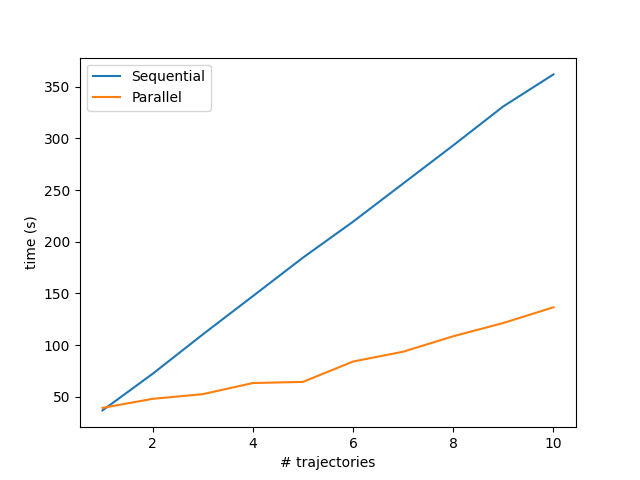
\includegraphics[width = \columnwidth]{times_multiprocessing}
    \centering
    \caption{Tempi di esecuzione - Sequenziale vs Parallelo}
    \label{fig:seq_vs_par}
  \end{figure}

  \subsection{NetworkGenerator}
  \paragraph{}
  La misurazione fa riferimento all'intera generazione della rete, e include quindi sia l'esecuzione 
  di \textit{generate\_graph} che quella di \textit{generate\_cims}. 

  \subsubsection{Tempi}
  \begin{figure}[H]
    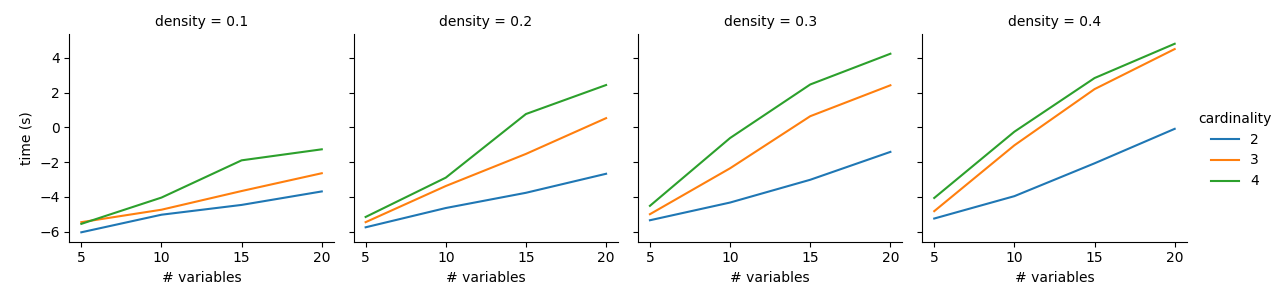
\includegraphics[width = \columnwidth]{times_network}
    \centering
    \caption{Tempi di esecuzione - NetworkGenerator}
  \end{figure}

  \paragraph{}
  È possibile osservare come i tempi seguano approssimativamente lo stesso andamento di quelli
  mostrati per la generazione delle traiettorie rispetto alla complessità della rete.
  Tuttavia, a parità di parametri, l'esecuzione dei metodi di \textit{NetworkGenerator} è
  un'operazione mediamente più veloce rispetto al campionamento di una traiettoria.

  \vspace{6mm}

  \begin{center}
    \begin{tabular}{c|cc|cccc}
      \toprule
      $\# \; variables$ & {} & {} & $d = 0.1$ & $d = 0.2$ & $d = 0.3$ & $d = 0.4$\\
      \midrule
      \multirow{3}{*}{5} & \multirow{3}{*}{\rotatebox[origin=c]{90}{card.}} & 2 & 0.0007 & 0.0008 & 0.0008 & 0.0012\\
      {} & {} & 3 & 0.0007 & 0.0015 & 0.0022 & 0.0025\\
      {} & {} & 4 & 0.0009 & 0.0015 & 0.0035 & 0.0055\\

      \midrule
      \multirow{3}{*}{10} & \multirow{3}{*}{\rotatebox[origin=c]{90}{card.}} & 2 & 0.0015 & 0.0045 & 0.0039 & 0.0025\\
      {} & {} & 3 & 0.0018 & 0.0250 & 0.0647 & 0.1290\\
      {} & {} & 4 & 0.0070 & 0.0165 & 0.8248 & 0.2829\\

      \midrule
      \multirow{3}{*}{15} & \multirow{3}{*}{\rotatebox[origin=c]{90}{card.}} & 2 & 0.0025 & 0.0061 & 0.0171 & 0.0219\\
      {} & {} & 3 & 0.0066 & 0.2312 & 0.7580 & 11.8190\\
      {} & {} & 4 & 0.0543 & 1.9960 & 10.0167 & 19.2014\\

      \midrule
      \multirow{3}{*}{20} & \multirow{3}{*}{\rotatebox[origin=c]{90}{card.}} & 2 & 0.0086 & 0.1340 & 0.0664 & 0.4041\\
      {} & {} & 3 & 0.0210 & 2.2293 & 9.5017 & 43.8563\\
      {} & {} & 4 & 0.1711 & 12.2124 & 22.9523 & 38.2674\\
      \bottomrule
    \end{tabular}
    
    \captionof{table}{Dev. Standard dei tempi di esecuzione - NetworkGenerator}
  \end{center}

  \subsubsection{Memoria}
  \begin{figure}[H]
    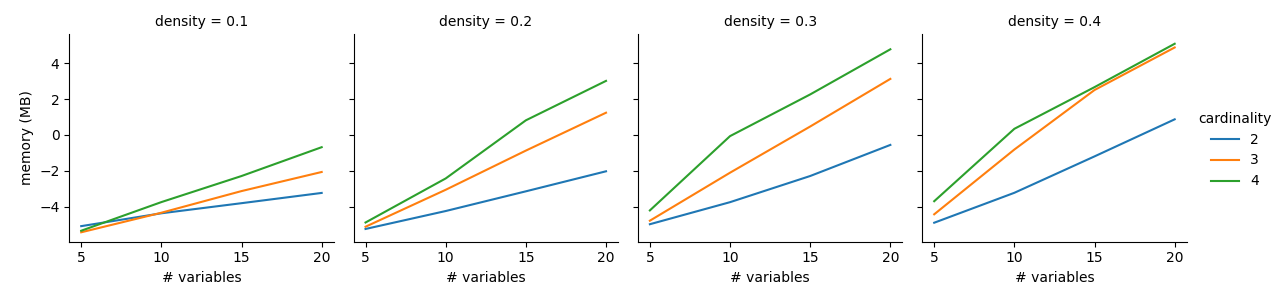
\includegraphics[width = \columnwidth]{memory_network}
    \centering
    \caption{Utilizzo della memoria - NetworkGenerator}
  \end{figure}

  \paragraph{}
  È possibile applicare un ragionamento analogo a quello presentato in relazione alla variabilità
  della memoria utilizzata nell'ambito del campionamento delle traiettorie. I valori più elevati
  si riscontrano infatti in corrispondenza delle densità maggiori, che significano un aumento della 
  probabilità che un nodo abbia più archi entranti, quindi un maggior numero di CIM che 
  riflettano tali dipendenze e come diretta conseguenza un aumento dello spazio occupato in RAM.

  \vspace{6mm}

  \begin{center}
    \begin{tabular}{c|cc|cccc}
      \toprule
      $\# \; variables$ & {} & {} & $d = 0.1$ & $d = 0.2$ & $d = 0.3$ & $d = 0.4$\\
      \midrule
      \multirow{3}{*}{5} & \multirow{3}{*}{\rotatebox[origin=c]{90}{card.}} & 2 & 0.0058 & 0.0006 & 0.0007 & 0.0006\\
      {} & {} & 3 & 0.0004 & 0.0003 & 0.0013 & 0.0038\\
      {} & {} & 4 & 0.0007 & 0.0009 & 0.0051 & 0.0074\\

      \midrule
      \multirow{3}{*}{10} & \multirow{3}{*}{\rotatebox[origin=c]{90}{card.}} & 2 & 0.0074 & 0.0007 & 0.0032 & 0.0064\\
      {} & {} & 3 & 0.0011 & 0.0244 & 0.0514 & 0.1300\\
      {} & {} & 4 & 0.0062 & 0.0304 & 1.3823 & 0.5247\\

      \midrule
      \multirow{3}{*}{15} & \multirow{3}{*}{\rotatebox[origin=c]{90}{card.}} & 2 & 0.0088 & 0.0072 & 0.2492 & 0.0561\\
      {} & {} & 3 & 0.0151 & 0.4742 & 0.6426 & 13.0242\\
      {} & {} & 4 & 0.0416 & 1.8642 & 6.2715 & 12.5361\\

      \midrule
      \multirow{3}{*}{20} & \multirow{3}{*}{\rotatebox[origin=c]{90}{card.}} & 2 & 0.0110 & 0.0170 & 0.1434 & 1.0643\\
      {} & {} & 3 & 0.0383 & 4.5907 & 10.5345 & 59.6651\\
      {} & {} & 4 & 0.3288 & 22.4537 & 36.4545 & 51.8351\\
      \bottomrule
    \end{tabular}

    \captionof{table}{Dev. Standard delle quantità di memoria occupata - NetworkGenerator}
  \end{center}
  
  \chapter*{Conclusioni}
  \label{chapter_conclusioni}
  \addcontentsline{toc}{chapter}{Conclusioni}
  \paragraph{}
  In relazione a quanto osservato è possibile affermare che gli obiettivi iniziali sono
  stati soddisfatti, dando un piccolo contributo allo sviluppo e alla crescita di
  PyCTBN. È stata inoltre mantenuta l'intenzione di rispettare i principi su cui è stata
  sviluppata la libreria, ricorrendo a scelte progettuali che garantissero la flessibilità
  e l'estensibilità del software, astraendosi completamente dal formato dei dataset e
  agevolando ulteriori integrazioni.\\
  Per garantire la qualità del lavoro, tutti i metodi sono stati approfonditamente testati
  con molteplici configurazioni, sperimentando inoltre l'interazione con le componenti già esistenti.
  Allo scopo di favorire la leggibilità, la manutenibilità e innanzitutto l'utilizzo dei
  moduli introdotti, è stata prodotta una documentazione riguardante tutte le classi, i metodi e i 
  relativi parametri, provvedendo inoltre a fornire un esempio pratico di realizzazione dell'intero flusso
  di esecuzione, che prevede la generazione della rete, il campionamento di una traiettoria
  su di essa, l'apprendimento della struttura a partire da tale traiettoria e infine 
  l'esportazione su file dei dati prodotti.\\
  Come già ampiamente sottolineato, la libreria rimane aperta all'introduzione di
  funzionalità aggiuntive che le possano conferire ulteriore completezza, rendendola
  un framework open-source consolidato per lavorare con le reti Bayesiane a tempo continuo.
  Si potrebbe pensare di allineare PyCTBN all'unica alternativa esistente, CTBN-RLE,
  implementando tutti i moduli non ancora presenti e superando le criticità prestazionali peculiari di quest'ultima.
  Alcune funzionalità significative sarebbero ad esempio legate all'inferenza su una rete
  e all'apprendimento con dati non completi.
  Un ulteriore miglioramento possibile, anche se non di banale realizzazione, consisterebbe
  nel prendere in considerazione la proprietà di faithfulness nell'ambito della generazione
  delle reti, che come spiegato nel relativo capitolo è stata attualmente trascurata.\\
  Per quanto riguarda il percoso di stage, è stata un'esperienza altamente formativa,
  che ha convogliato molte delle competenze acquisite nel corso del triennio,
  dando inoltre una dimostrazione dell'applicazione pratica di concetti finora
  ristretti alla sola teoria. È stata anche l'occasione di un primo approccio al 
  mondo della ricerca, cercando di trarre il più possibile dalla competenza, dall'esperienza e dalla
  passione dimostrate da chi mi ha guidato in questo lavoro, fornendomi spunti e
  consigli con grande disponibilità.

  \nocite{*}
  \bibliographystyle{unsrt}
  \bibliography{main}
\end{document}